\chapter{Choosing a \texorpdfstring{\gls{co2}}{CO2} Sensing Technique}\label{chap:choosing_techno}

\begin{tldrbox}
	
	The specifics of transcutaneous \gls{co2} sensing revealed in the previous chapter are used to select an appropriate \gls{co2} sensing technique for this particular location. Thin-film dye-based \gls{co2} sensing is opted for, and both the associated chemistry and potential optical sensing schemes are presented. \Gls{fdlr} is finally chosen and its mathematical intricacies are briefly exposed, outlining the need for an accurate phase shift measurement between two---potentially noisy---sinusoidal signals. This latter mathematical problem is then studied in-depth, reaching a practically-interesting solution that highlights a power consumption / accuracy compromise. This chapter lays the theoretical foundations that will be applied in practice in the next one.
	
	\tcblower
	
	\hyperref[chap:tcco2]{Previous chapter} \hfill \hyperref[chapter:toc]{Main Table Of Content (TOC)} \hfill \hyperref[chap:thin_film]{Next chapter}
	
\end{tldrbox}
\glsreset{fdlr}

\vspace{.3cm}\hrule\vspace{.1cm}\hrule\vspace{.3cm}

Ce qu'on avait dit pour le chpitre d'avant: DLR 
chimie de mesure en film fin épisode I (choix polymères / fluorophores), chimie de mesure en film fin épisode II (capteur en lui-même)

Ce que j'ai fait: j'ai divisé ça en deux entre ce chapitre et le précédent. On avait oublié la partie revue des technos de mesure du CO2. Ça donne donc plutôt :
- choix d'une techno de mesure
- principe de cette techno de mesure dans le détail
- le DLR + mesure de phase

\vspace{.3cm}\hrule\vspace{.1cm}\hrule\vspace{.3cm}

With the previous chapter outlining the main characteristics of transcutaneous \gls{co2} sensing, the next step is to choose a \gls{co2} sensing technique that aligns with these specificities. In this view, the present chapter begins with a massive literature review of \gls{co2} sensing techniques in Section~\ref{sect:choos:sensors_review}---itself corresponding to Section~2 of our previous Sensors review article\cite{dervieux2022}. Then, the conclusions of the previous chapter are put in perspective with the former review, in order to select what seems to be the most appropriate sensing technique in a transcutaneous sensing context. This is done in Section~\ref{sect:choos:techno_choice}, itself partially inspired by Section~4 of the afore-mentioned article\cite{dervieux2022}. The chosen technique---dye-based \gls{co2}-sensitive thin films---is then discussed in more detail in Section~\ref{sect:choos:dye_based}, outlining the possible use of an interesting sensing scheme termed \gls{dlr}. The latter calls for an accurate phase measurement from a noisy sinusoidal signal, which is the very topic of Section~\ref{sect:choos:phase_mes}---itself based on our \hl{APSIPA Transactions on Signal and Information Processing} paper\hl{[666]}.

\section{Review of \texorpdfstring{\gls{co2}}{CO2} Sensing Techniques}\label{sect:choos:sensors_review}

Fortunately, since \gls{co2} is ubiquitous in our world, its measurement has been the goal of many researchers from very different fields, each with their own constraints and objectives. In particular, \gls{co2} sensing is used: in the food storage and agri-food industry\cite{acock1995}, in medical science\cite{severinghaus1986_3}, in sea and environmental research\cite{shitashima2010}, and of course in the laboratories themselves---\eg{} analytical chemistry. Such a diversity of applications leads to different constraints in terms of operating conditions---such as temperature and pressure---cost, durability, maintenance, \textit{etc.}

Yet, our aim is not to produce in these pages a complete bibliographic review of each and every one of the mentioned techniques. We do so for the sake of conciseness, and because comprehensive reviews focusing on one or another of the techniques presented below are available in the literature\cite{fanget2011, zosel2011, puligundla2012, llobet2013, neethirajan2009, barrington2018, rebber2020, rezk2020, bhowmick2020}. While the latter perform an in-depth coverage of their respective topic---\eg{} nanomaterials-based sensors\cite{llobet2013, rezk2020}---they never cover the full spectrum of \gls{co2} sensing possibilities. This is partly done, however, in the book \emph{Carbon Dioxide Sensing}\cite{decker2019}, which covers certain aspects of the present work in much more details, although letting others aside, and to which the curious reader may refer to quench their curiosity.

The present review spans the full range of \gls{co2} measuring techniques with the exception of the analytical ones. That is for instance (mass) spectroscopy, magnetic resonance, chromatography, or titration. We did so because such techniques are not likely to be used for biomedical monitoring in the near future, due to the bulky and expensive apparatus they require. These methods are covered in-depth by dedicated analytical chemistry works, though\cite{skoog2013, harvey2016}.

For each technique reviewed, the underlying physical principle enabling \gls{co2} measurement is exposed briefly. Such explanations are often accompanied by a clear figure or schematic to allow for a rapid comprehension of the presented technique. The main features, advantages, and drawbacks of the technique are also disclosed, with typical characteristics of commercial or research applications, when available or relevant. The aim of such summaries is to provide the reader with a basic understanding of each exploited phenomenon, while giving them references to research articles or reviews to dig further. At the end of this section, a table is also given to summarise all the presented techniques and to compare them on several merit criteria---\eg{} lifetime, accuracy, drift, cross-sensitivities, response time, form factor, \etc{}.---see Section \ref{subsect:choos:review:comp_table}.

The structure of this review is organized around the physico-chemical properties of the \gls{co2} molecule, namely:
\begin{enumerate}
	\item[--] The infrared absorption of \gls{co2}---Section \ref{subsect:choos:ir_abs}.
	\item[--] The hydration of dissolved \gls{co2} into carbonic acid---Section \ref{subsect:choos:review:hydration}.
	\item[--] The reduction of \gls{co2} into \ce{CO^-_2} and \ce{CO^2-_3}---Section \ref{subsect:choos:review:reduction}.
	\item[--] The acoustic properties of gaseous \gls{co2}---Section \ref{subsect:choos:review:acoustic}.
\end{enumerate}

\subsection{Infrared Absorption of \texorpdfstring{\gls{co2}}{CO2}}\label{subsect:choos:ir_abs}

\subsubsection{\texorpdfstring{\gls{ndir}}{NDIR} Sensors}\label{subsect:choos:review:ndir}

The operating principle of \gls{ndir} \gls{co2} sensors is that of the Beer-Lambert law of absorption, for gaseous \gls{co2} exhibits an absorbance peak at 4.26~\textmu{}m, as can be seen in Figure \ref{fig:choos:review:ndir_gas_spectra}. Due to the absence of other commonly encountered gases absorbing at this wavelength, \gls{ndir} sensors are very specific and can reach extremely low levels of detection if the sensing cavity is long enough. They operate as follows: an infrared source is placed on one end of a cavity containing the gaseous analyte, while an infrared receptor is placed at the other end. At a given wavelength $\lambda$, the measured light flux $\Phi_\text{mes}$ (W) is then function of: the emitted light flux $\Phi_0$ (W), the geometry of the sensor $k$ (unit-less), the light path length $l$ (m), the \gls{co2} volume fraction $\chi_{\ce{CO_2}}$ (unit-less), and its absorbance $\mathcal{A}_{\ce{CO_2}}$ (m$^{-1}$) following\cite{bernath1995}

\begin{equation}
	\Phi_\text{mes}(\lambda) = k \cdot \Phi_0(\lambda) \cdot 10^{- l \cdot \chi_{\ce{CO2}} \cdot \mathcal{A}_{\ce{CO_2}}(\lambda)}
\end{equation}

\begin{figure}
	\centering
	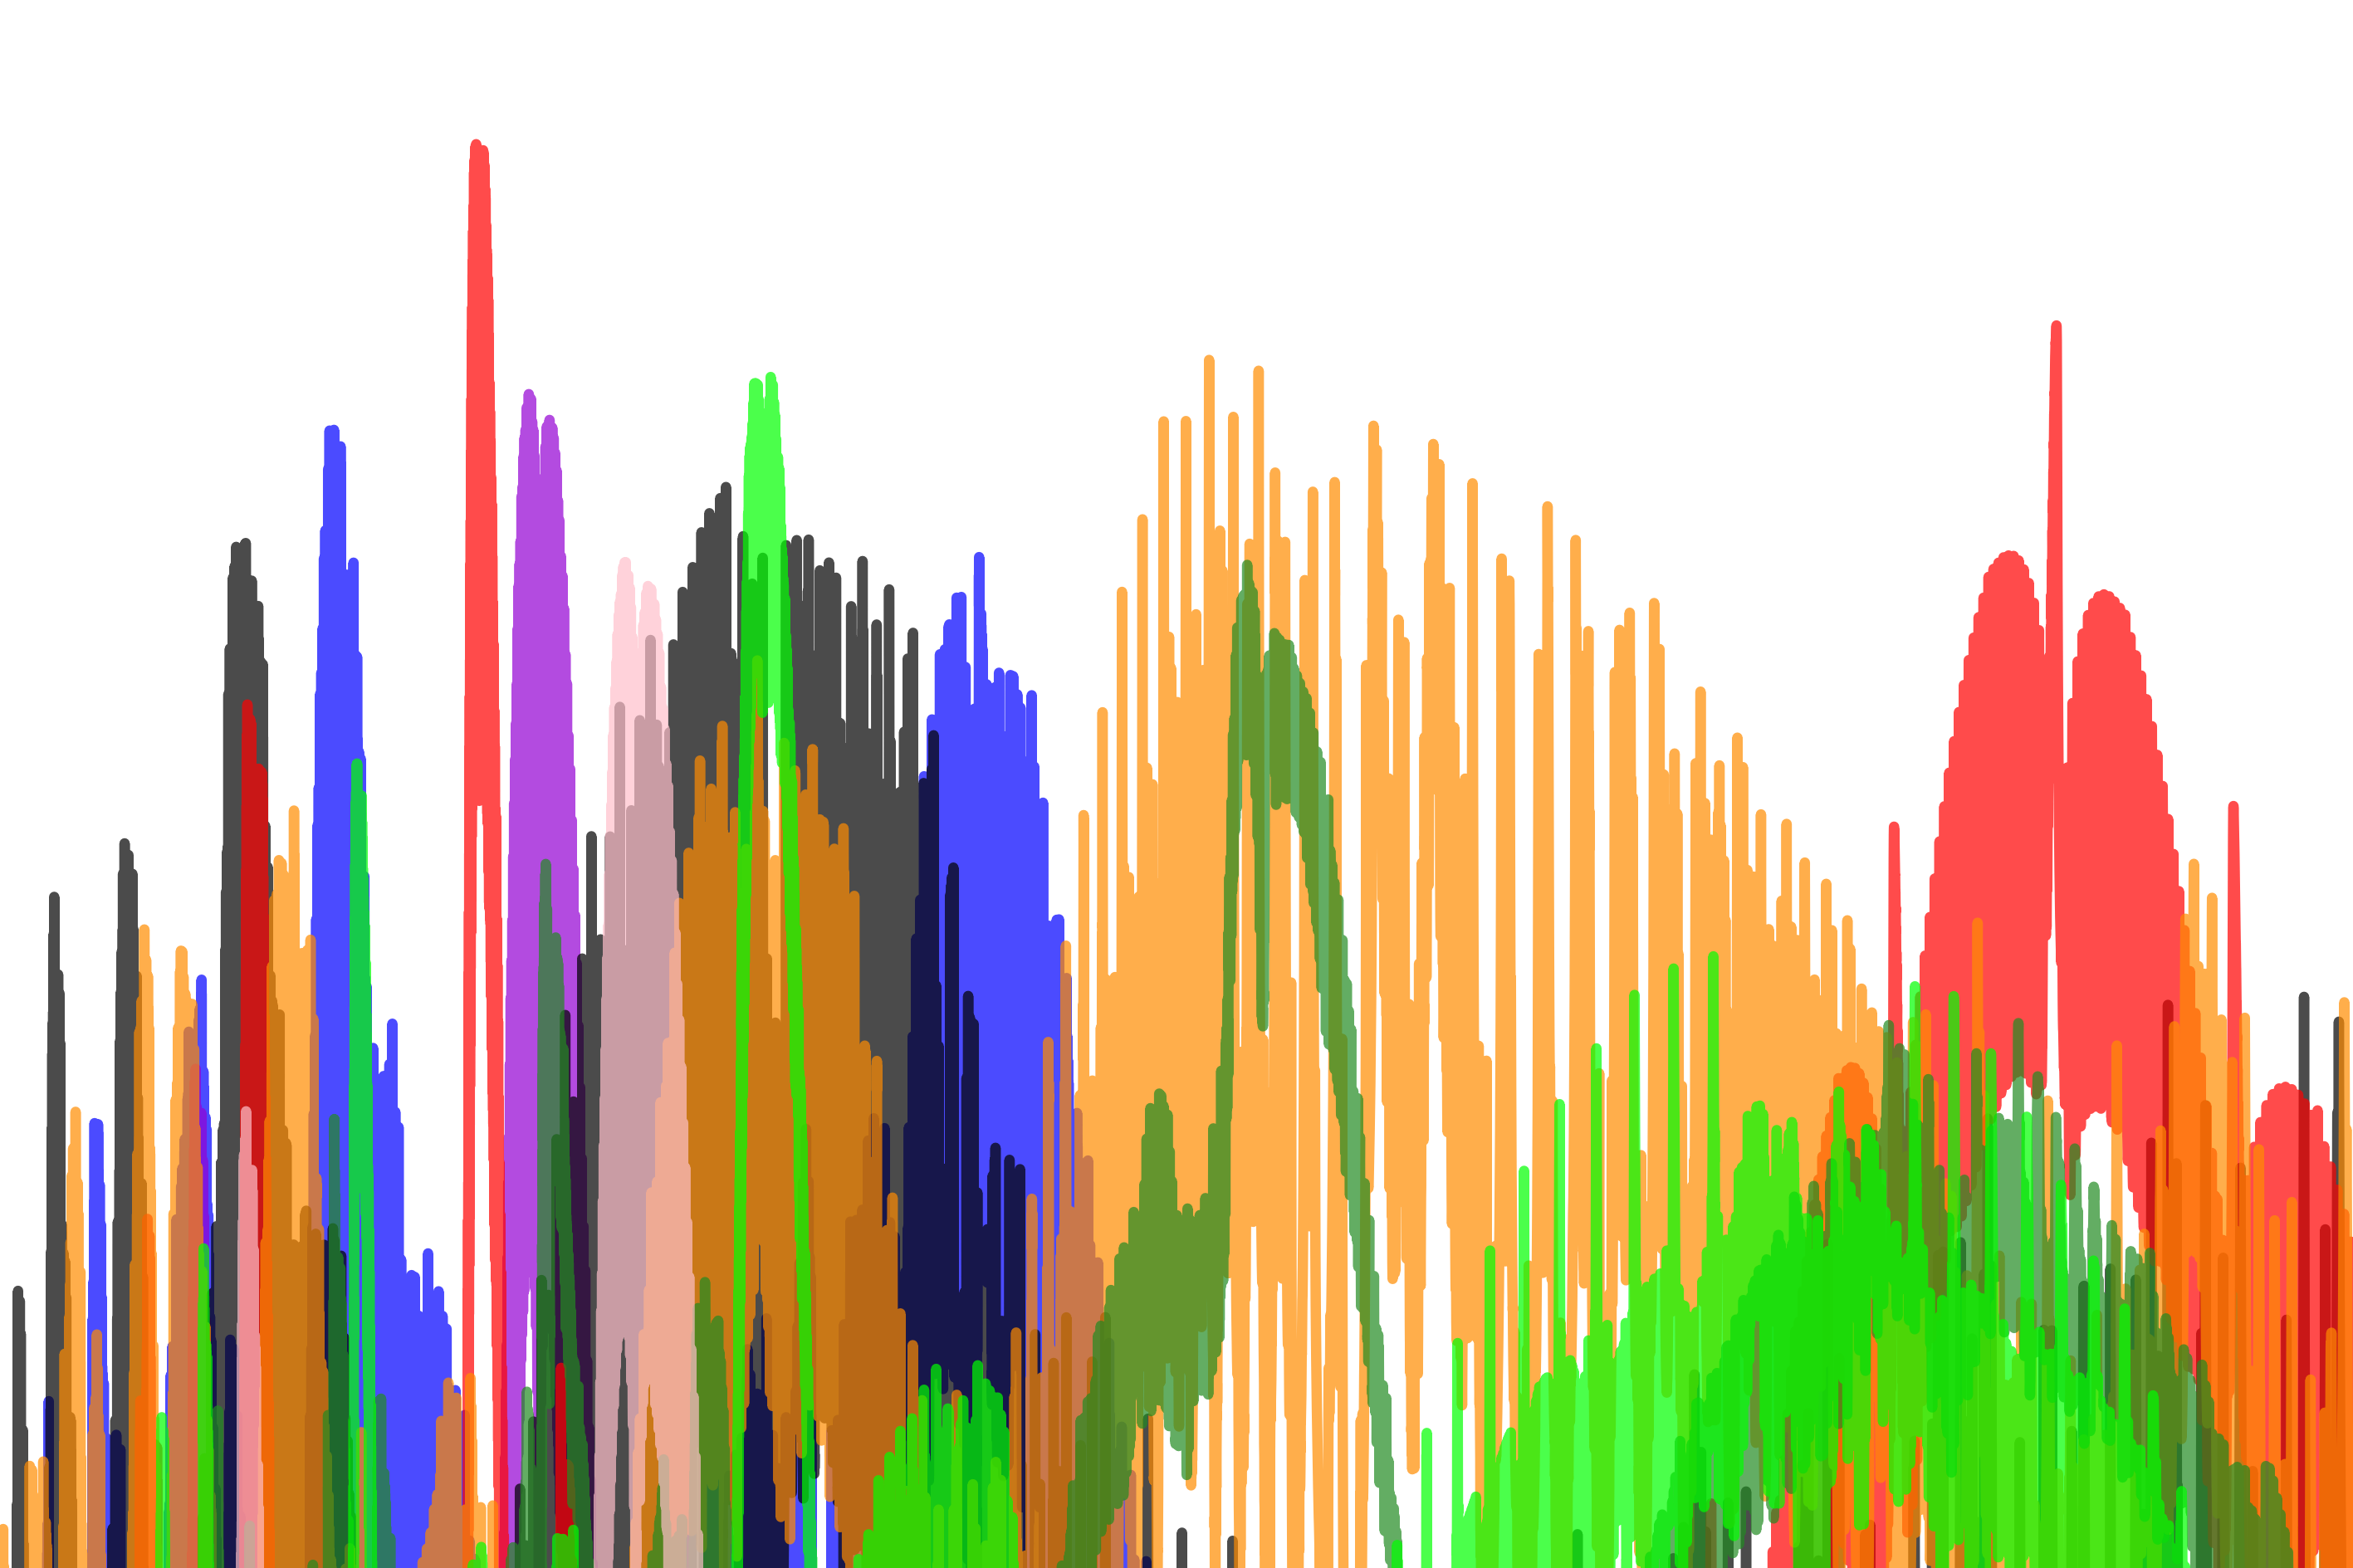
\includegraphics{1_main_matter/choos_figures/review/tikz/out/ndir_gas_spectra.pdf}
	\caption[Mid infra-red absorption spectra of various gases.]{Mid infra-red absorption spectra of various gases, only \gls{co2} absorbs at 4.26~\textmu{}m. Data source: HITRAN database\cite{hitran2017}. A Lorentzian broadening profile was considered for a dilution in air at 1~atm and 296~K.}
	\label{fig:choos:review:ndir_gas_spectra}
\end{figure}

While this equation indicates a linear relationship between $\log_{10}(\Phi_\mathrm{mes}/\Phi_{0})$, $l$, and $\chi_{CO_2}$, the actual linkage between the latter quantities is generally much more difficult to model accurately, due to a variety of light paths that contribute differently to the sensor response. Although this plurality of light paths can be studied beforehand by simulation---as did Hodgkinson, Liu \etal{}\cite{hodgkinson2012, hodgkinson2013, liu2016}---most sensors are calibrated empirically once manufactured.

Theoretically, only one emitter / receiver duo is needed, given that one of them is narrow-band---or bandpass filtered---around 4.26~\textmu{}m, so as to avoid interferences from other gases. In practice however, a \emph{reference} channel is often placed beside the \emph{measurement} one\cite{popa2019, zhang2010, jing2020}. The role of this additional reference channel is to compensate for fluctuations in the light source intensity due to temperature variations, for instance. In this case, the sensor is composed of two sensing elements, one is covered by a 4.3~\textmu{}m bandpass filter, while the other one is covered by a bandpass filter in the 3.8--4.1~\textmu{}m region, where no other gas absorbs. Other designs have also been proposed using a time-interleaved reference / measurement channel alternation, instead of two physically distinct light paths. In this case, a single sensing element is covered by a rotating filter wheel equipped with multiple bandpass filters at 4.2~\textmu{}m and 3.8~\textmu{}m\cite{kohsiek1991}. The typical design of such referenced sensors is presented in Figure \ref{fig:choos:review:ndir_sensor_scheme}, Left.

\begin{figure}
	\centering
	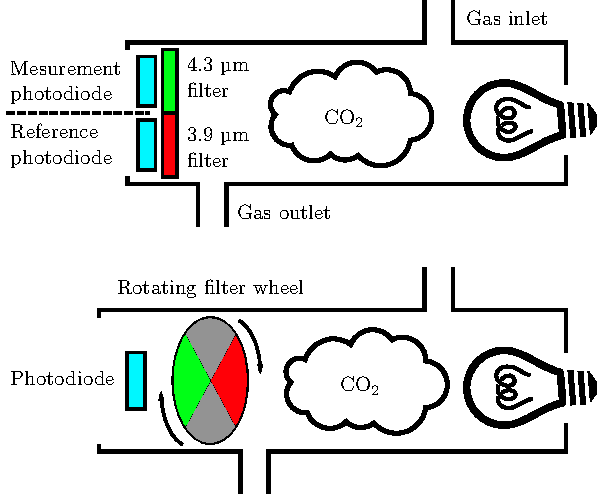
\includegraphics[valign=c,width=.55\linewidth]{1_main_matter/choos_figures/review/ndir_outline_converted}
	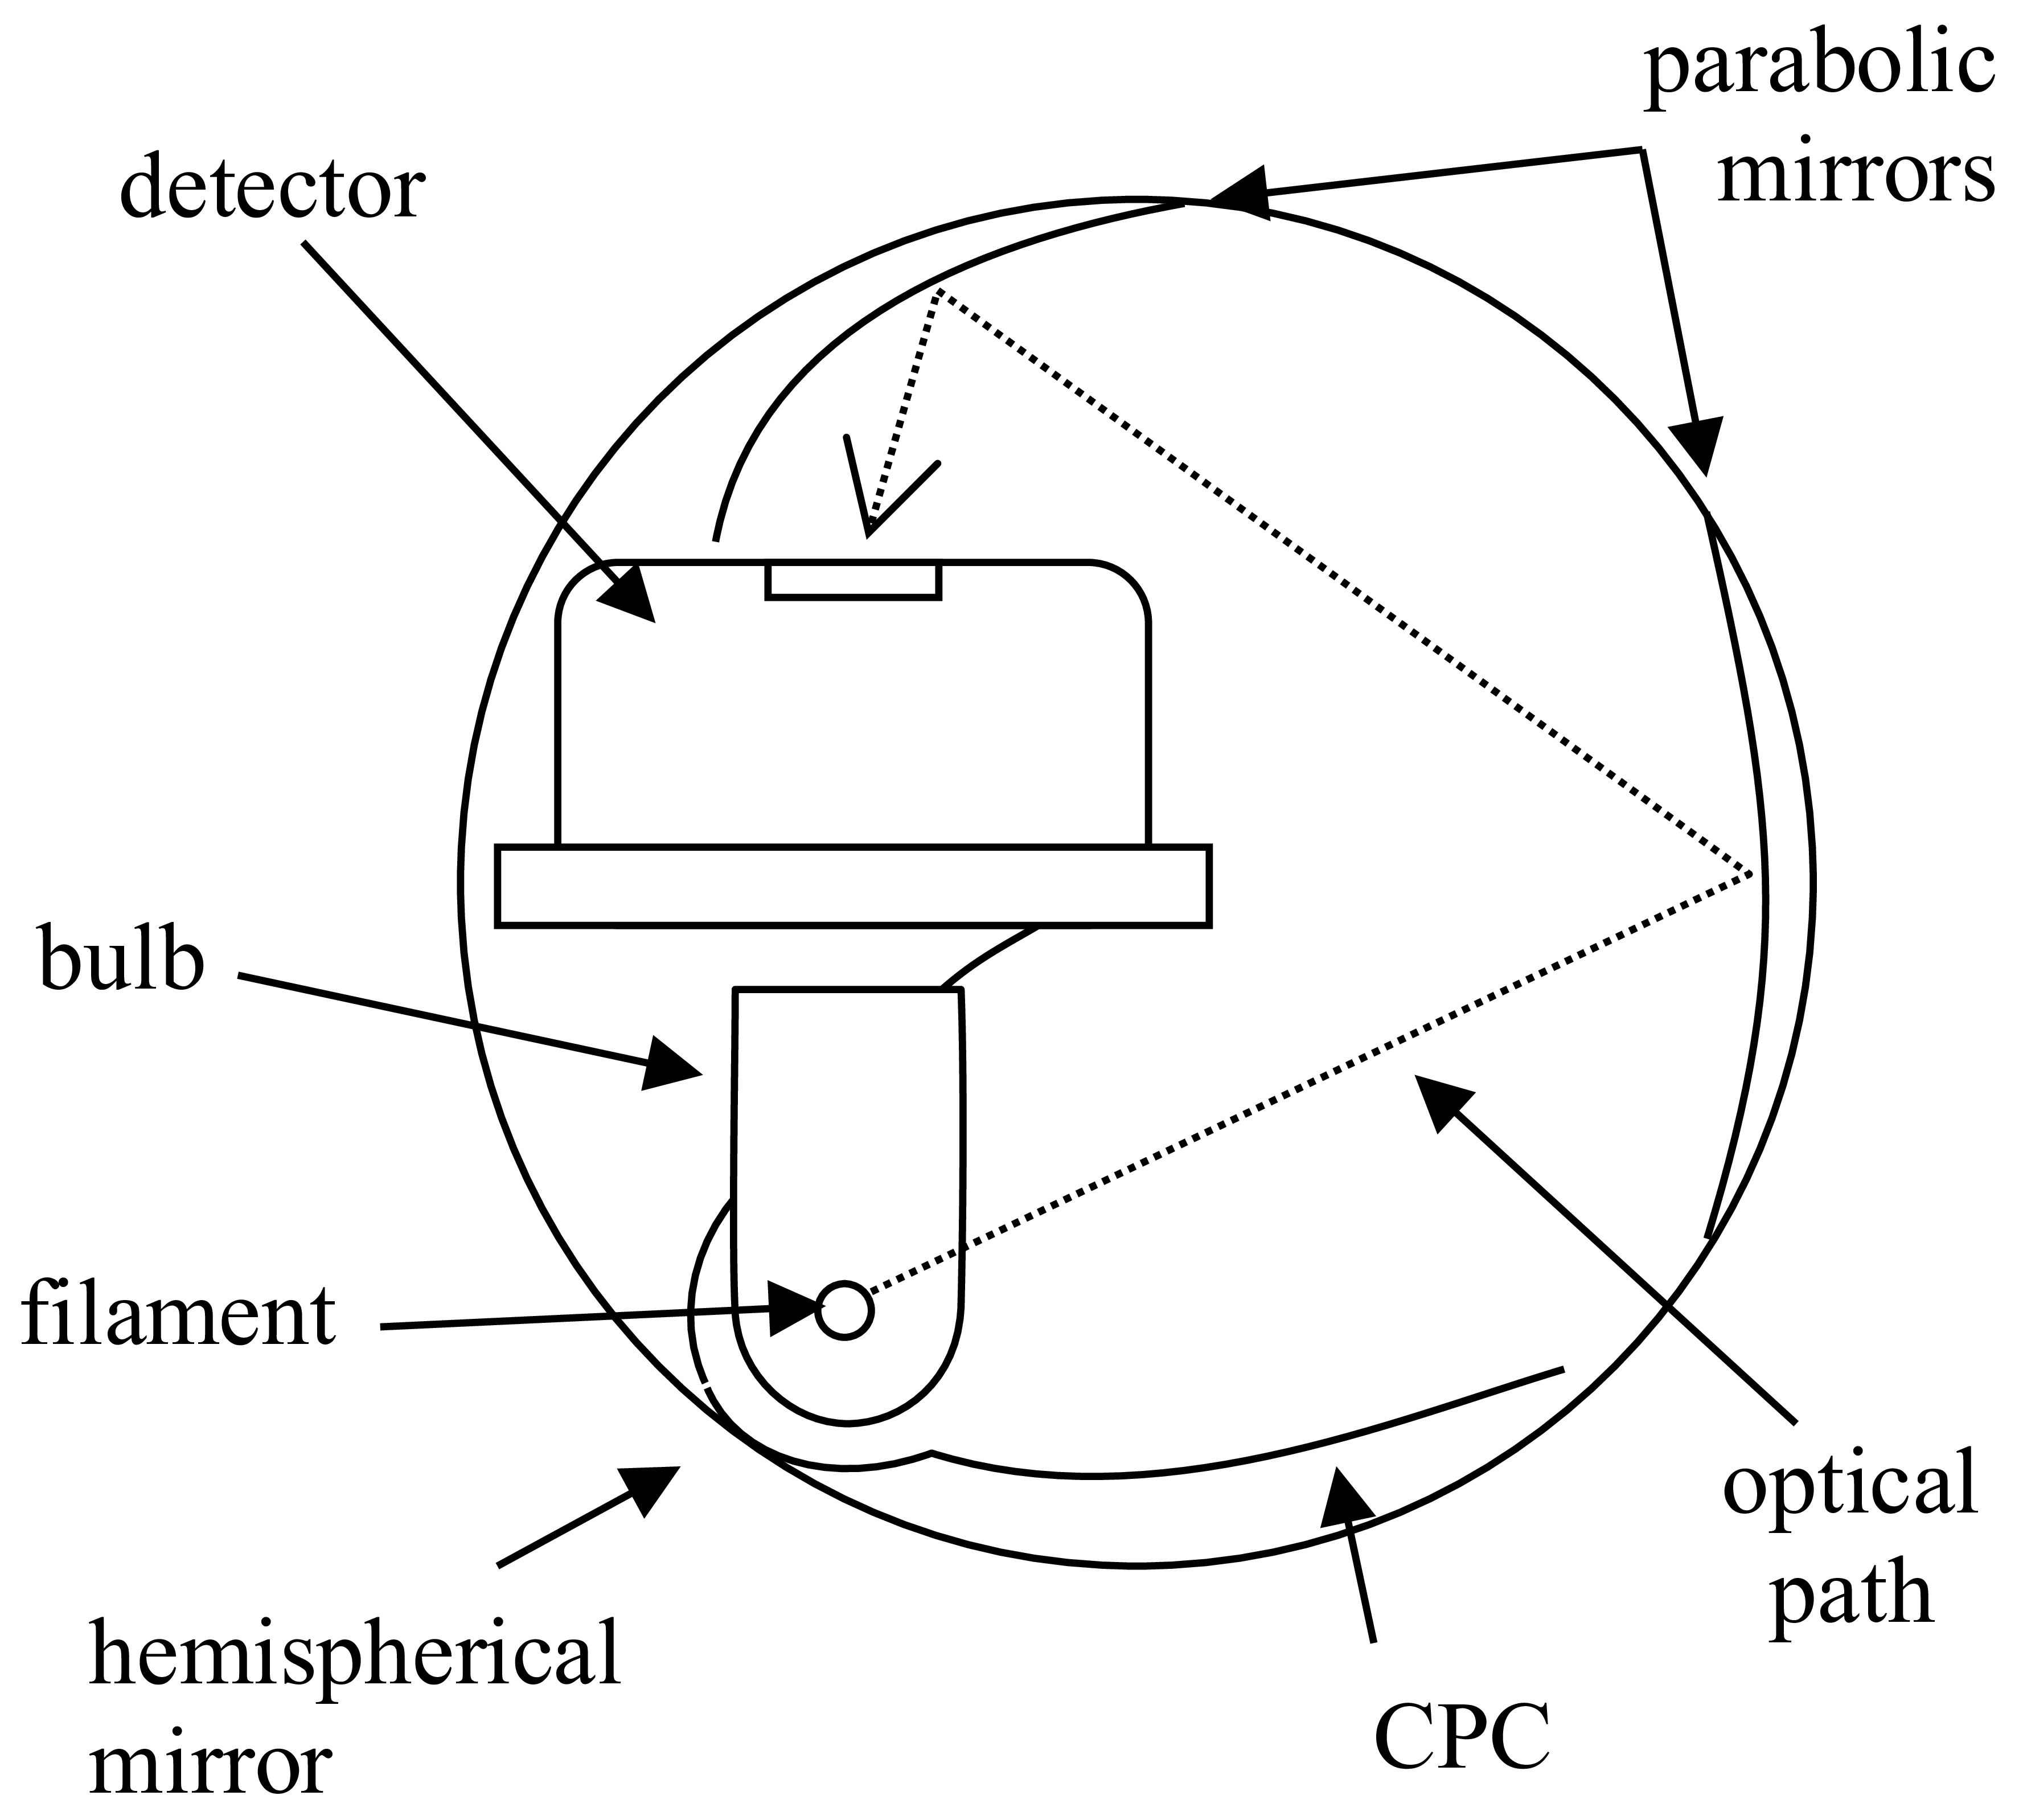
\includegraphics[valign=c,width=.44\linewidth]{1_main_matter/choos_figures/review/ndir_long_path}
	\caption[\gls{ndir} sensors outlines.]{\textbf{Left:} outline schematic of a space-interleaved (top) and time-interleaved (bottom) \gls{ndir} \gls{co2} sensor. In the time-interleaved sensor, a rotating filter wheel acts as a chopper, with two opaque sectors, and two sectors equipped with 4.3~\textmu{}m and 3.9~\textmu{}m bandpass filters, respectively. \textbf{Right:} a more complex design allowing for longer light paths in a compact device. The detector has two channels, a measurement and a reference one, as in the upper left scheme. CPC stands for Compound Parabolic Collector, a type of light concentrator. Reproduced with permission from Hodgkinson \etal{}\cite{hodgkinson2013}.}
	\label{fig:choos:review:ndir_sensor_scheme}
\end{figure}

\gls{ndir} sensors were often criticised because of the infrared source they used---{\ie} a bulb with a heating filament---which both consumed much power and generated heat\cite{gibson2013}. However, with recent advances in the domain of infrared emission and sensing, this is no longer a source of concern. In particular, recent InAsSb semi-conductors allow for reasonably cheap and energy efficient emitters and receiver, {\eg} AK9700AE (\gls{led}) and AK9710 (sensor), AKM, Japan, or Lms43 \gls{led} and photodiode, LMSNT, Russia. Alternatively, thermopiles---possibly miniaturised as \gls{mems}---also offer good alternatives to the aforementioned photodiodes\cite{xu2017}. Similarly, \gls{mems} emitter have also been developed\cite{lee2009, liu2016}.

The response time of \gls{ndir} sensors is limited by the gas flow rate into the sensing chamber, while their sensing range is essentially a function of their light path. Thus, it is possible to create fast sensors with operating ranges going from a few hundreds ppm up to 100\% \gls{co2}\cite{gibson2013, vincent2016}. It should be noted however, that since the detection of small concentrations requires long light path---up to 80~mm for 100~ppm for instance\cite{vincent2016}---it can lead to bulky sensors. In order to solve the latter issue, more complex sensing geometries can be envisioned to lengthen the light path while keeping a compact sensor, as can be seen in Figure \ref{fig:choos:review:ndir_sensor_scheme}, Right. Additionally, while \gls{ndir} \gls{co2} sensors are not sensitive to relative humidity levels below 100\%\cite{kohsiek1991, gibson2013}, condensation can lead to the formation of water droplets, either in the light path as fog, or on the surface of light emitters, receivers, or reflectors, thus disturbing the measurements\cite{vincent2016, muller2020}\footnote{This issue was also mentioned in Section~\ref{subsect:tcco2:gas_tightness} regarding the onset of condensation inside the gold-plated dome of the \gls{ndir} sensor that was used for transcutaneous \gls{co2} conductivity measurements.}. Fortunately, this latter issue may be solved by either detecting potential dew-point situations and removing potentially polluted measurements\cite{wang2018}, or heating the sensor itself, though at the cost of a higher power consumption\cite{fietzek2014, gss_condensation}.

Reviews of mid-infrared sources\cite{jung2017}, \gls{ndir} applications for gas sensing in general\cite{hodgkinson2012rev, popa2019}, and concrete applications to \gls{co2} measurement\cite{zhang2010, hodgkinson2013, moumen2016, vincent2016} can all be found in the literature. Interestingly, even if predominantly reported in the gas phase, \gls{ndir} \gls{co2} measurements may also be performed onto an aqueous solution containing dissolved \gls{co2}\cite{schaden2004}.

\subsubsection{Photoacoustic Sensors}\label{subsect:choos:review:photoacous}

Photoacoustic sensors also use the afore-mentioned absorbance of \gls{co2} in the mid infrared (4.26~\textmu{}m), and periodically illuminate the \gls{co2} present inside a given sensing volume. Either a mechanical chopper with a continuous source, a low-inertia pulsating source, or even a pulsed laser is used to produce a periodic infrared illumination on the gas sample to analyse. If \gls{co2} is present in the gas mixture, it absorbs the infrared radiation and thus heats up, dilating slightly. When the illumination is stopped, the mixture cools down and thus compresses. An alternating illumination thus causes a repetition of these dilatations and compressions, which is nothing more than an acoustic wave. The latter can in turn be measured with a microphone\cite{bozoki2011}.

This technique requires a light source that can be modulated at high frequencies---depending on the geometry of the cell and the sensor used---which is achievable using \glspl{led} or lasers, but precludes the use of a light bulb as an infrared light source---unless a mechanical chopper is used, of course. Depending on the targeted accuracy or measurement range, several designs may be employed. The simplest one consists in a non-resonant acoustic cell with a basic microphone and light modulated in the 20~Hz--20~kHz range\footnote{Since this range corresponds to human hearing, many microphones are available off-the-shelf in this frequency band.}. However, using a resonant cell design and placing the microphone at an antinode of the acoustic wave can lead to much higher output levels. Such a design is illustrated in Figure \ref{fig:choos:review:pipe_acous} with an organ-pipe-like resonant cell. With cells in the centimetre range, this translates into frequencies below 40~kHz. Further still, the microphone can consist in a quartz tuning fork---a piezoelectric transducer with a quality factor above 10~000.

\begin{figure}
	\centering
	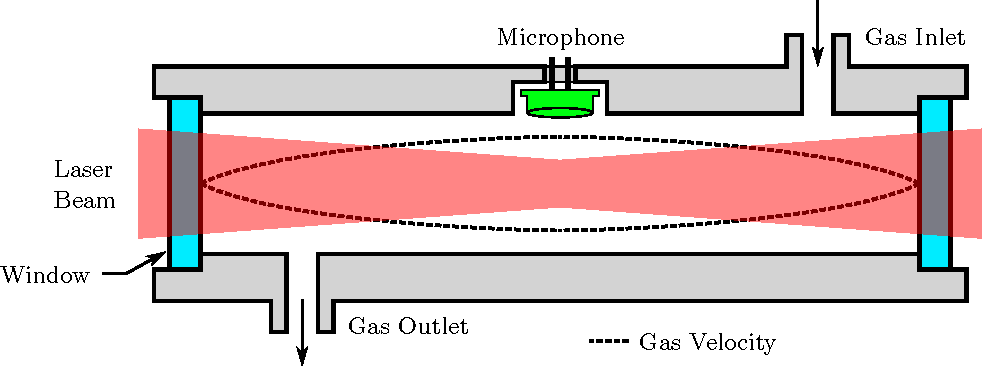
\includegraphics[width=\linewidth]{1_main_matter/choos_figures/review/photoacous_pipe}
	\caption[Outline schematic of an organ-pipe-like resonant acoustic cell.]{Outline schematic of an organ-pipe-like resonant acoustic cell. The cell consists in a pipe closed at its two ends with optical windows. A laser beam at 4.26~\textmu{}m is then pulsed at the resonant frequency of the pipe, which forms a $\lambda/2$ resonator. For instance, if a 32,768~Hz quartz tuning fork is used as a microphone, $\lambda\approx10$~mm and a pipe length of $\sim$5~mm would be ideal. A velocity-sensitive microphone may be placed at half the pipe as depicted. Alternatively, a pressure-sensitive microphone would rather be placed near one of its ends.}
	\label{fig:choos:review:pipe_acous}
\end{figure}

With the use of resonant photoacoustic cells or microphones---\eg{} quartz tuning forks---very high sensitivities of a few ppm or even ppb can be achieved\cite{borri2014}. Yet, quartz tuning forks are influenced by temperature and humidity---even if this cross-sensitivity is reproducible and can thus be compensated for---and may need to be frequently recalibrated\cite{rousseau2019}. Contrariwise, \gls{mems} microphones appear to be independent of humidity---even if being temperature-sensitive---and no frequent calibration need was reported\cite{scholz2017}. Abundant examples of photoacoustic sensors can be found in the literature\cite{huber2015, pernau2016, scholz2017} and recent research is ongoing, targeting their miniaturisation into \gls{mems} sensors\cite{lhermet2019}. Besides, photoacoustic \gls{co2} sensors can be designed for the full range of \gls{co2} sensing---from a few ppb up to 100\% \gls{co2}---and their response time is mainly limited by the gas flow inside the sensor. It should be noted that this flow is necessarily limited, since high flow value generates turbulences, which are essentially acoustic noise\cite{bozoki2011}.

\subsection{Hydration of \texorpdfstring{\gls{co2}}{CO2} into Carbonic Acid}\label{subsect:choos:review:hydration}

As mentioned in Section~\ref{subsect:co2hb:bicarb}, when presented to an aqueous medium, gaseous \gls{co2} dissolves into carbonic acid (\ce{H_2CO_{3,(aq)}}), which further dissociates into bicarbonate (\ce{HCO^-_{3,(aq)}}) and carbonate (\ce{CO^{2-}_{3,(aq)}}) ions, following\cite{jensen1979, mills2009}:

\begin{equation}\label{eq:choos:rev:co2_diss}
	\ce{CO_{2,(aq)} + H2O <=>[\textit{K}_1][] H2CO_{3,(aq)}} \quad \begin{cases}
		K_1 = 1.5\cdot 10^{-3} \\
		\text{p}K_1 = 2.8
	\end{cases}
\end{equation}
\begin{equation}\label{eq:choos:rev:h2co3_diss}
	\ce{H_2O + H_2CO_{3,(aq)} <=>[\textit{K}_2][] H_3O^+_{(aq)} + HCO^-_{3,(aq)}} \quad
	\begin{cases}
		K_2 = 4.44\cdot 10^{-7} \\ \text{p}K_2 = 6.35
	\end{cases}
\end{equation}
\begin{equation}\label{eq:choos:rev:hco3_diss}
	\ce{H_2O + HCO^-_{3,(aq)} <=>[\textit{K}_3][] H_3O^+_{(aq)} + CO^{2-}_{3,(aq)}} \quad
	\begin{cases}
		K_3 = 4.67\cdot 10^{-11} \\ \text{p}K_3 = 10.33
	\end{cases}
\end{equation}
wherein typical values of $K_\text{i}$ can be found in the literature\cite{millero2006, wang2010} and are given here in pure water at 25{\degree}C. The consequences of such dissociations are twofold: first, \gls{co2} dissolution tends to lower the pH of the aqueous medium; second, the presence of dissolved ions induces changes in the conductance of the solution. While the former phenomenon is the basis for the functioning of the \ssel, \gls{isfet} sensors and dye-based sensors, the latter one enables conductometric \gls{co2} sensors to operate.

\subsubsection{Wet Conductometric Sensors}\label{subsect:choos:review:wet_conduct}

Wet conductometric sensors take advantage of the fact that when \gls{co2} dissolves into an aqueous solution, \ce{HCO^-_3} and \ce{H_3O^+} ions are produced, which in turns modify the conductivity of the solution\cite{baker1996}. A typical static conductometric sensor is composed of a chamber filled with distilled water and containing two electrodes. The chamber is then covered with a \gls{co2}-permeable membrane to allow outer \gls{co2} to diffuse inside the sensor\cite{varlan1997, mirtaheri2004a, mirtaheri2004b}. Alternatively, a dynamic conductometric sensor may be build, into which distilled water is circulated between a gas diffusion area and an impedance measurement area\cite{acock1995, baker1996}. A static measurement cell is depicted in Figure \ref{fig:choos:review:conduct_outline}. Using such an apparatus, the sensing medium may be either liquid or gaseous, while dynamic flow-through geometries have only been reported using gaseous analytes.

\begin{figure}
	\centering
	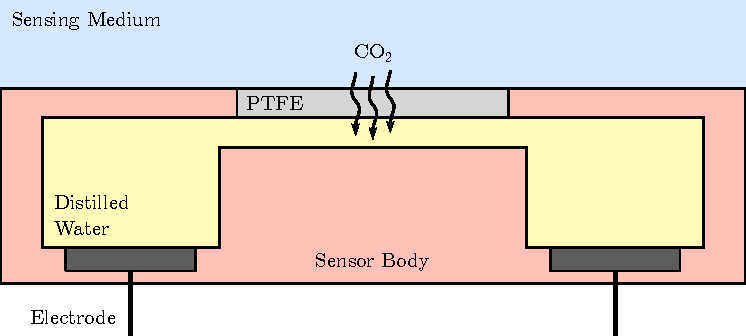
\includegraphics{1_main_matter/choos_figures/review/wet_conduct}
	\caption[Outline of a static conductometric cell.]{Outline of a static conductometric cell. \gls{co2} diffuses into distilled water, modifying the concentration of H$_3$O$^+$, HO$^-$ and HCO$_3^-$ and thus the conductivity of the solution, which may be measured using alternative current to avoid polarisation by mean of two electrodes.}
	\label{fig:choos:review:conduct_outline}
\end{figure}

Such sensors are in theory inexpensive, easy to build, and stable. In practice however, a drift is often observed whose roots are not accurately known, even if some authors suggest a contamination of the distilled water with external ions. In particular, if glues or resins are used to attach the membrane to the sensor, or to assemble the different parts of the embodiment together, they may suffer from outgassing and release ions in the distilled water\cite{mirtaheri2004a}. If the membrane is not tightly sealed, foreign ions originating from the sensing medium may also enter the solution, and thus change its conductivity. Drift correction\cite{tronstad2010} or automatic recalibration\cite{wall1995a} techniques have thus been developed to compensate for this phenomenon. Alternatively, other authors immersed the body of their electrode for at least two weeks in bi-distilled water to make sure that foreign ions possibly bound to the glass surface of their sensor re-dissolve in the rinsing water and are thus eliminated\cite{lis1979}. The dynamic flow-through geometry also eludes this issue by forcing the water into a de-mineralizing resin while being recycled.

As is the case for other membrane-covered sensors---see Section \ref{subsect:choos:review:ssel} below, for instance---the water can still evaporate through the covering membrane depending on the ambient relative humidity, especially in the case of static sensors used on a gaseous analyte. This issue was partially addressed by Neethirajan \etal{}\cite{neethirajan2010}, who presented a \gls{ptfe} membrane-covered sensor using Nafion as a proton conductor over a layer of polyaniline boronic acid, which exhibits a conductivity change upon a change in its pH. Using this contraption, the authors reported a relatively stable response for \gls{rh} levels in the 20--70\% range. Overall, wet conductometric \gls{co2} sensor can be used on the full 0--100\% \gls{co2} range, with response times below 1~min. Still their usable lifetime has not been reported in the literature and may be seriously impacted by the afore-mentioned drift.

\subsubsection{The Stow-Severinghaus Electrode}\label{subsect:choos:review:ssel}

The \ssel---named after its inventors Richard Stow\cite{severinghaus1986_3} and John Severinghaus\cite{severinghaus1958}---is the current state-of-the-art method for transcutaneous \gls{pco2} sensing\cite{conway2018}. Even if it has been miniaturised since its first introduction, its basic working principle remains unchanged. As one can see in Figure \ref{fig:choos:review:ssel_outline}, it is nothing more than a pH-meter plunging in an electrolyte and covered with a thin membrane. Originally designed for \emph{ex vivo} blood \gls{pco2} sensing, it was later modified to be used transcutaneously as well\cite{beran1976}.

\begin{figure}
	\centering
	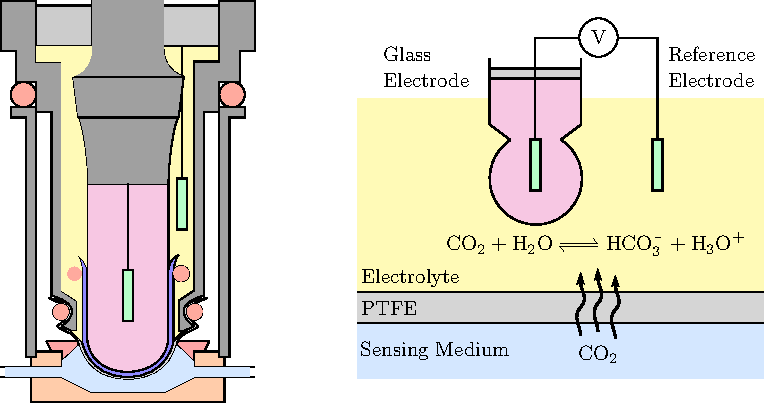
\includegraphics{1_main_matter/choos_figures/review/ssel_converted}
	\caption[The Stow-Severinghaus electrode.]{\textbf{Left:} the Severinghaus electrode, an improvement of the Stow electrode, as first described in the 1958 publication\cite{severinghaus1958}. The colour of the different elements matches that of the simplified schematic on the right. \textbf{Right:} outline schematic of the Severinghaus electrode. \gls{co2} diffuses through a \gls{ptfe} membrane into an electrolyte, causing a change in the pH of the latter. Such a change is then recorded by the mean of a pH-meter that consists of a glass electrode and a reference electrode.}
	\label{fig:choos:review:ssel_outline}
\end{figure}

Dissolved \gls{co2} diffuses from the outer medium into the sensor's embodiment through a thin membrane, made of an ion-impermeable and \gls{co2}-permeable material. A rubber membrane was originally proposed but was quickly replaced by a \gls{ptfe} one\cite{severinghaus1986_3, severinghaus1958}, although silicone rubber is still occasionally used for its ease of application and better adhesion\cite{shin2000}. The electrolyte was also switched from distilled water to a solution of sodium carbonate (NaHCO$_3$) and sodium chloride (NaCl) in various concentrations that influence both the sensitivity and response time of the electrode\cite{jensen1979}. \gls{co2} dissociation lowers the pH of the electrolyte---as described by Equations~\ref{eq:choos:rev:co2_diss}--\ref{eq:choos:rev:hco3_diss}---which is then measured using a pair of electrodes: the glass electrode, and the reference electrode. The glass electrode consists in an Ag/AgCl electrode more often than not, although a Sb/SbO$_x$ electrode has also been occasionally reported\cite{beran1976}, while the reference electrode can be made of Pt\cite{severinghaus1958, severinghaus1981} or AgCl\cite{beran1976}. Alternatives to the glass electrode have been explored with liquid membranes instead of the traditional glass bulb\cite{zhao1997}, or a replacement of the whole electrode by an iridium oxide film grown electrochemically on an iridium wire, yielding a higher sensitivity and being reportedly easier to manufacture than the glass electrode\cite{suzuki1999, beyenal2004}.

Apart from miniaturisation and the exploration of other membrane materials, redox electrode pairs, or pH membrane material, the electrode underwent little changes compared to its original design. The response time of the \ssel{} is generally reported to lie in the 1--5~min range, although the addition of carbonic anhydrase---a catalyst to the reaction \ref{eq:choos:rev:co2_diss}---led to response times below 1~min\cite{donaldson1979, shin2000}. Still, the long-term stability of the electrode rarely exceed a few months and some amount of drift is always present, making necessary to re-calibrate the electrode every few hours or days, depending on the targeted accuracy\cite{zhao1997, mcguire2002}. The full range of the \ssel{} is usually that of physiological \gls{pco2} levels---\ie{} $\sim$2.6--13.2~kPa (or $\sim$20--100~mmHg)\cite{conway2018}---although applications for concentrations as low as $\sim$0.05--0.1\% ($\sim$0.5~mmHg) have also been reported\cite{cai1993, zhao1997}. The temperature dependency of the electrode may be compensated for, and a mixture of water and ethylene glycol can be used as a base for the electrolyte, preventing the electrode from drying out from a loss of water vapour through the gas-permeable membrane\cite{whitehead1980}.

\subsubsection{\texorpdfstring{\gls{isfet}}{ISFET} Sensors}\label{subsect:choos:review:isfet}

\glsreset{isfet}
Due to the limited miniaturisation potential of the \ssel, \glspl{isfet} were explored as \gls{co2} sensing devices. \glspl{isfet} are \gls{mosfet} whose gate is \ce{H_3O^+} sensitive. The addition of a reference electrode can turn them into compact---yet fully functional---pH-meters. The use of \gls{isfet} for pH sensing has been reported as early as 1970\cite{bergveld1970} and was later extended to \gls{co2} sensing with the addition of a layer of bicarbonate solution covered with a gas-permeable, ion-impermeable, silicone rubber membrane\cite{hu1989}.

\begin{figure}
	\centering
	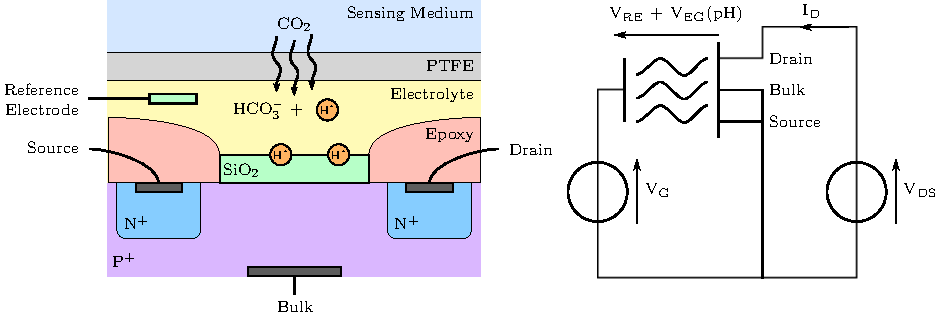
\includegraphics[width=\linewidth]{1_main_matter/choos_figures/review/isfet_converted}
	\caption[\gls{isfet} sensors.]{\textbf{Left:} outline schematic of an \gls{isfet} \gls{co2} sensor. \gls{co2} diffuses from the analyte inside the inner electrolyte through a \gls{ptfe} membrane, changing the pH of the electrolyte and generating hydronium ions (abbreviated H$^+$). The ions will penetrate the upper layer of the porous SiO$_2$ gate insulator, influencing the P$^+$ substrate underneath, and thus the conductance of the transistor. \textbf{Right:} basic electrical implementation schematic of an \gls{isfet} sensor. The actual grid-source potential seen by the transistor is the sum of the applied grid voltage V$_\text{G}$, the voltage between the reference electrode and the electrolyte V$_\text{RE}$, and that between the electrolyte and the gate insulator V$_\text{EG}$, itself function of the pH of the electrolyte.}
	\label{fig:choos:review:isfet}
\end{figure}

As can be seen in Figure \ref{fig:choos:review:isfet}, the \gls{isfet} gate insulator is not metallised but rather covered with a layer of silicon oxide (SiO$_2$), itself optionally covered with another layer of silicon nitride (Si$_3$N$_4$), hafnium oxide (HfO$_2$), aluminium oxide (Al$_2$O$_3$) or tantalum pentoxide (Ta$_2$O$_5$). Once hydrated, the upper layer of the gate insulator becomes able to exchange protons with the surrounding electrolyte, thus acting as a pH electrode. Still, another electrode---the reference electrode---is needed to apply or measure a grid-source potential on the transistor. This latter potential---$V_{GS}$---itself function of the pH of the electrolyte, modulates the conductance of the transistor, hence turning it into a pH sensor\cite{bergveld1981}. \gls{co2} detection can then be performed by covering the electrolyte with a \gls{co2}-permeable membrane, impermeable to other ions. This basic approach has been successfully applied by a number of authors in the literature, either for pH measurements\cite{hu1989, jamasb2019}, or direct \gls{co2} sensing\cite{star2004, mohri2006, shitashima2010, ekwinska2012}.

Among the above-mentioned gate insulators, hafnium oxide offers better performances in terms of drain current, sensitivity and body effect than silicon nitride. Hafnium oxide may even be used alone, in place of the silicon oxide layer\cite{lai2010}. The inner electrolyte usually consists in a bicarbonate solution, while the reference electrode is often an AgCl / Ag electrode. \gls{isfet} \gls{co2} sensors are subject to the same drawbacks as the \ssel, namely the drift of the reference electrode and temperature dependency, although the latter may be compensated for. An approach for drift correction has also been proposed with good results either on restrained\cite{jamasb2019} or wide pH ranges\cite{sinha2020}. The dry-out and humidity sensibility problems have been addressed with a dry sensor\cite{shimanoe2004}, even if the drift of the latter has yet to be reported. Alternatively, a low-drift design with a deported reference electrode has also been proposed with promising results\cite{hsieh2014}.

\subsubsection{Dye-Based Sensors}\label{subsect:choos:review:dye_based}

Dye-based \gls{co2} sensors also rely on the influence of \gls{co2} hydration and dissociation on the pH of an aqueous solution. The pH change caused by the dissociation of \gls{co2} translates into a change in the optical properties of a pH-sensitive dye, which can exist in either a protonated---AH---or an anionic---\ce{A^-}---form. The dye is chosen so that its protonated and anionic forms differ either in their absorbance or luminescence spectra, and also for having a \Ka{} acidity constant near that of reaction \ref{eq:choos:rev:h2co3_diss} ($\pKa=-\log_{10}(\Ka)\approx6.3$ in water at 25{\degree}C\cite{macinnes1933}). This dye can either be dissolved in an aqueous solution---which is in turn entrapped between a substrate layer and a gas-permeable, ion-impermeable membrane---or dissolved in a thin polymer film with the aid of a phase transfer agent. These two kinds of sensors are often referred to as \enquote{wet} and \enquote{dry} sensors, respectively. A typical fluorescent sensor is depicted in Figure \ref{fig:choos:review:dye_based}, along with the fluorescence spectra of \gls{hpts}---a commonly encountered pH-sensitive fluorophore---at different \pH{} values.

\begin{figure}
	\centering
	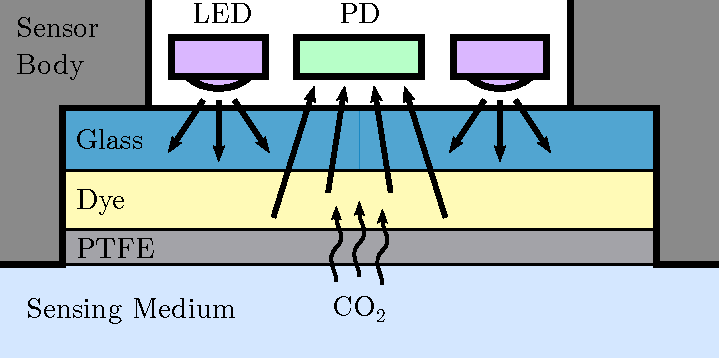
\includegraphics[valign=c, width=0.51\textwidth]{1_main_matter/choos_figures/review/dye_sensor}
	\hspace{0.2cm}
	\includegraphics[valign=c]{1_main_matter/choos_figures/review/tikz/out/hpts_uttamlal1995}
	\caption[Dye-based sensors outline.]{\textbf{Left:} outline schematic of a typical dye-based \gls{co2} sensor. The \glspl{led} illuminate a pH-sensitive dye, either dissolved in an aqueous solution or a polymer, through a layer of transparent substrate---here a glass slide. The dye is protected from ionic contamination by a \gls{ptfe}, gas-permeable, ion-impermeable membrane. The \glspl{led} and photodiode (PD) may additionally be covered by excitation or emission filters in case of fluorescence measurement. \textbf{Right:} the fluorescence excitation spectra of 1~mM \gls{hpts} in carbonated distilled water equilibrated with different \gls{pco2} values. Data source: Uttamlal \etal{}\cite{uttamlal1995}.}
	\label{fig:choos:review:dye_based}
\end{figure}

The most basic sensors use a single wavelength for illumination---in case of absorbance measurements---or a pair of excitation-emission wavelengths---in case of luminescence measurement. Photobleaching may be compensated for, using more wavelengths and ratiometric methods similar to that driving pulse oximetry\cite{vurek1983, uttamlal1995, degrandpre1999, ge2003, lu2008, hakonen2008, ge2014, wang2020}, while variations in the emitted light intensities or sensitivities toward received light can be addressed by using referencing---\ie{} taking a measurement in pure \gls{n2} and / or pure \gls{co2} prior to \gls{co2} measurement for sensor calibration purposes\cite{opitz1984, zhujun1984b, wolfbeis1988, he1995, marazuela1995, mills1997, malins1998, wolfbeis1998, segawa2003, oter2006, fernandezsanchez2007, oter2008, chu2008, chu2009, dansby2010, chu2017, perez2017}.

\glsreset{dlr}
Three other more sophisticated sensing schemes have been developed through the years, in addition to the afore-mentioned techniques, using an additional pH-independent, reference florescent dye: namely the \gls{ife}, \gls{dlr} and \gls{fret}. Those techniques are presented in more detail in literature reviews or research articles focusing either on dye-based sensors in general\cite{mills2009, clarke2017} or on specific applications such as the \gls{ife}\cite{nakamura2003, amao2004, amao2005a, amao2005b, perez2009, aguayolopez2014, fernandezramos2018, fernandezramos2019}, \gls{dlr} measurements\cite{klimant2001_pap, bultzingslowen2002, burke2006, cajlakovic2006, fritzsche2017, staudinger2018, pfeifer2020} or \gls{fret}\cite{lakowicz1993, neurauter1999, valeur2001_chap9, bultzingslowen2003}. Surprisingly, none of these methods appears to be notably better than another, with some state-of-the-art works using either \gls{dlr}\cite{pfeifer2020}, \gls{ife}\cite{fernandezramos2018} or simple referencing\cite{chu2017}.

In contrast, a clear distinction exists between dry and wet sensors, with dry sensors largely outperforming wet ones, would it be in terms of response time, long-term stability, or ease of manufacturing\cite{wolfbeis2005, mills2009}. Dry sensors are basically made out of a substrate layer, onto which a polymer is cast. The dye(s) of interest is prior dissolved into the polymer by mean of a phase transfer agent before casting. A plasticiser is also often added to enhance the \gls{co2} diffusion inside the polymer layer. Optionally, the latter may be covered by an additional protective layer, so as to prevent ionic contamination, or destruction of the sensor by acidic vapours. Apart from the optical sensing scheme, the main differences between the many dry sensors mentioned in the literature lie in the choice of the substances used for the aforementioned layers. Although no exhaustive comparison can be found, several authors compared different combinations of chemicals:

\begin{enumerate}[leftmargin=*,labelsep=4.9mm]
	\item	\textbf{Substrate:} the substrate material does not seem to have any major influence on the sensing performance and is indifferently made of \gls{pet} films, glass slides, or optical fibers. Nonetheless, \gls{pen} appears to be superior to \gls{pet}, because its lower diffusivity towards \gls{co2} yields shorter response times\cite{fritzsche2017}. In addition, the adhesion of the polymer film on glass substrate can be difficult without a cumbersome surface preparation\cite{cajlakovic2006, dansby2010} while \gls{pen} foils may just be roughened to enhance the sensitive layer adhesion\cite{fritzsche2017}.
	\item	\textbf{Polymer:} \gls{hpmc} may be a better choice than ethyl cellulose for being more hydrophilic than the latter, allowing water molecules to be entrapped with the dye and favouring the hydration of \gls{co2} into bicarbonate ions\cite{aguayolopez2014}.
	\item	\textbf{Plasticiser:} several plasticisers were compared in the literature, \gls{tbp} and Tween 20 appear to be the most efficient ones in terms of sensor response time\cite{wolfbeis1998, aguayolopez2014}.
	\item	\textbf{Phase transfer agent:} \gls{ctah} tends to lead shorter response times\cite{bultzingslowen2002} although \gls{tmah} may be more stable since it is less susceptible to Hofmann elimination\cite{aguayolopez2014}.
	\item	\textbf{Covering membrane:} Hyflon or even Cytop may be used if a minimal response time is not mandatory, in order to limit the sensor poisoning and humidity loss\cite{fritzsche2017}.
\end{enumerate}

Overall, dye-based sensors cover the full 0--100\% \gls{co2} range with response times below 1~min---a few seconds have even been seldom reported\cite{amao2005b, chu2008, chu2017}---accuracies below 1\%, lifetimes approaching one year\cite{fernandezramos2018, fernandezramos2019} and thicknesses as low as 1~\textmu{}m\cite{dansby2010}. Still, they may be destroyed quickly by acidic vapours, and often suffer from a high cross-sensitivity towards humidity, \gls{o2}---for it is a fluorescence quencher\cite{kautsky1939, lakowicz1973}---and temperature. While a protective membrane may mitigate the first two drawbacks, temperature influence may be compensated for. \gls{o2} cross-sensitivity can also be reduced, either by using polymers with a low oxygen permeability\cite{perez2009, fernandezramos2018} or by entrapping the \gls{o2}-sensitive luminophore inside polystyrene micro- or nano-beads\cite{huber2000, bultzingslowen2002, cajlakovic2006}. Using a dual frequency \gls{dlr} scheme may also be relevant to compensate for \gls{o2} luminescence quenching\cite{klimant2001_pap}.

\subsubsection{Optical Fiber Sensors}\label{subsect:choos:review:fibre_optic}

Although optical fibers have been used in some of the afore-mentioned dye-based sensors to convey light back and forth between bulky bench-top equipments and compact sensing membranes or solutions\cite{he1995, lu2008, degrandpre1999}, they did not consist in the \gls{co2}-sensitive part itself. On the contrary, optical fibers-based \gls{co2} sensors put optical fibers at the very heart of their sensing principle, using one of the four different techniques presented in Figure \ref{fig:choos:review:fibre_optic}. These four sensing schemes can be grouped in two categories : either \textit{(i)} the \gls{co2} sensitive material changes the total light path length by shrinking or dilating in response to a change in \gls{co2} concentration and thus turns the optical fiber into a miniaturised Fabry-Perrot interferometer (case (b)), or \textit{(ii)} the \gls{co2} sensitive material exhibits a change in its refractive index or exert a mechanical constraint on the fiber core. In these last two cases, changes are made to the evanescent modes of the fiber, introducing a shift in the transmitted or reflected wavelengths (cases (a), (c) and (d)).

\begin{figure}
	\centering
	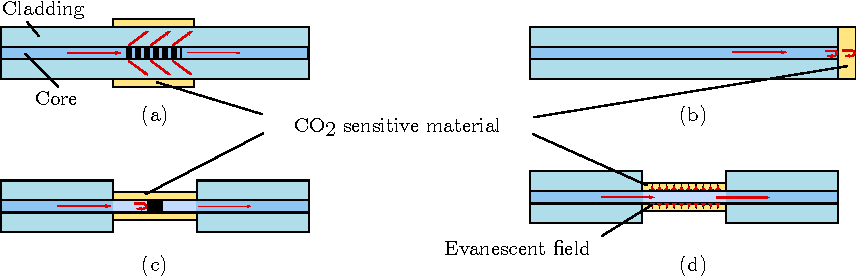
\includegraphics{1_main_matter/choos_figures/review/fibre_optics_barrington}
	\caption[Fibre optic sensor variations.]{\enquote{Various techniques that have been employed in \gls{co2} sensors to cause light propagating in the core to interact with the surrounding environment: (a) [Long Period Grating]; (b) extrinsic Fabry-Perot cavity; (c) [Fiber Bragg Grating] and; (d) etched cladding. All the examples here use a material which demonstrates \gls{co2} sensitivity and the subsequent change in coating upon exposure to \gls{co2} is sensed by the interacting light} -- Text and figure reproduced with permission from Barrington\cite{barrington2018}.}
	\label{fig:choos:review:fibre_optic}
\end{figure}

The principle behind end-of-fiber Fabry-Perrot interferometer-based sensors is to measure the interferences between the light wave reflected by the fiber-film interface and that reflected by the film-analyte interface. Depending on the wavelength of the probing light and the thickness of the film, the interferences can be either constructive or destructive, causing notches and peaks in the observed reflected spectrum. The exact positions of those spectral features are directly linked to the thickness of the film, and the latter fluctuates with the surrounding \gls{pco2}. Thus, accurate spectral measurements of the shift in wavelength of a given notch can yield reliable \gls{pco2} measurements\cite{zheng2015, ma2018}.

As for evanescent modes-based fibers, several sensing modalities exist. Fiber Bragg gratings may be used as a strain gauge on a block of pH-sensitive hydrogel that swells or contract with pH changes, thus bending the fiber it is attached to\cite{quintero2010}. Applying a mechanical strain on the optical fiber modifies its effective refractive index\cite{hill1997}, inducing a wavelength shift in the evanescent modes of the grating. This technique does not require an optical fiber in itself, however, since a regular pressure sensor may be used instead, possibly much cheaper and more convenient to implement\cite{herber2004}. The pH-sensitive hydrogel can also directly coat the optical fiber optic, with similar consequences, exerting strain on it\cite{hu2015}. Other materials, which exhibit a direct change in their refractive index upon \gls{co2} adsorption, have also been explored for optical fiber coating---such as metal organic frameworks or ionic liquids---with some success\cite{hromadka2018, barrington2018}.

Alternatively, other optical fiber-based sensors have been developed relying on principles closer to \gls{ndir} absorption than \gls{co2} hydration. Those utilise the absorption of evanescent waves by \gls{co2} present in the air surrounding the fiber at $\sim$1.5~\textmu{}m, where \gls{co2} absorbs. An additional coating of the fiber was shown to greatly improve the sensitivity of such sensors towards \gls{co2}\cite{melo2014, chong2015}.

% Evanescent coating + etching: chong, melo
% LPG : hromadka
% RI change : hu
% info PVA/PAA swelling : manavite

The main drawback of optical fiber-based sensors---apart from the elevated price tag of the measurement apparatus they requires---is their cross-sensitivity towards external strain, temperature, relative humidity, and possibly other chemicals which can be adsorbed by the optical fiber coating. Those sensors exhibit response time in the order of 1~min on the full 0--100\% range\cite{barrington2018, chong2015}. To our knowledge, the accuracy of such \gls{co2} sensors was never characterised extensively, although Melo \etal{}\cite{melo2014} measured a 4.1\% resolution on the full scale. Of note, if multiple sensors are used in the same facilities or geographical area, multiplexing can be used to share the light source and measurement apparatus between them, thus greatly reducing the cost per sensor\cite{kersey1993}. Such a multiplexing was demonstrated for probing up to 256 sensors on the same fiber, and distances as high as 150~km were reported\cite{perezherrera2013}.

% 1min 20% barrington2018
% 1min 500ppm-100% chong
% 110s 500-40000ppm hromadka2018
% 3min 50-650ppm ma2018
% X 0-100% melo2014 (reso 4%)

\subsection{Reduction of \texorpdfstring{\gls{co2}}{CO2}}\label{subsect:choos:review:reduction}

Sensors based on the reduction of \gls{co2} into \ce{CO^-_2} and \ce{CO^2-_3} radicals operate following several schemes
\begin{itemize}
	\item[--] \gls{co2} may be reduced following its adsorption on a thin film of metal oxide, thus modifying the conductivity of the oxide layer---Section \ref{subsect:choos:review:metal_oxide}.
	\item[--] A similar adsorption mechanism has also been reported between \gls{co2} molecules and gra\-phene, leading to graphene-based sensors---Section \ref{subsect:choos:review:graphene}.
	\item[--] Alternatively, the reduction of \gls{co2} may be used in an electrochemical cell, whose electromotive force yields the surrounding \gls{co2} activity---Section \ref{subsect:choos:review:electrochem_cell}.
	\item[--] Lastly, ionic liquids have also been used in \gls{co2} sensing, either binding to \gls{co2} to form carbamate species in conductometric sensor, or acting as a substrate for \gls{co2} reduction to peroxydicarbonate ions in amperometric sensors---Section \ref{subsect:choos:review:ionic_liquids}.
\end{itemize}

\subsubsection{Adsorption by Metal Oxide Thin Film}\label{subsect:choos:review:metal_oxide}

Adsorption-based sensors use the change in conductivity of a thin layer of metal oxide caused by the adsorption of \gls{co2}. Although the latter adsorption has been studied for a number of years\cite{hotan1979, au1988, freund1996, seiferth1999, lopesmartins2004}, its mechanism is still not entirely understood and remains a discussed topic in the scientific community\cite{herran2009, noei2011, tang2013, usseinov2019}. Indeed, both physical adsorption and chemisorption appears to take place at the metal oxide interface, and the reduction of \gls{co2} into \ce{CO^-_2} may not be the only mechanism involved\cite{tang2013}. That being said, the following reaction is often considered in the absence of a more satisfactory alternative\cite{gankanda2016, colak2019, alvarez2020}:
\begin{equation}
	\begin{aligned}
		\ce{CO_{2,(gas)} + e^- &<=> CO^-_{2,(ads)}} \\
		\ce{CO^-_{2,(ads)} + O^-_{(lat)} &<=> CO^{2-}_{3,(ads)}}
	\end{aligned}
\end{equation}
wherein \emph{ads} stands for \emph{adsorbed}, \emph{lat} for \emph{lattice}, and the O$^-$ radicals and $e^-$ are supposed to come from the MO lattice---where M may be Zn or Cu, for instance. Overall, despite the use of metal oxide \gls{co2} sensors by an important number of authors, few of them propose an explicit sensing scheme, and even fewer mind using equilibrated or justified schemes, which may lead to incoherences. For instance, it has been proposed that since the above-mentioned scheme consumes free electrons from the MO lattice, fewer of them remain available for conductivity\cite{kannan2014}. The resulting expected behaviour would be an increase in the metal oxide resistance with an increase in \gls{pco2}. While this assertion seems to hold in the simple ZnO case\cite{haeusler1996, kannan2014, colak2019}, opposite behaviours were observed when doping ZnO with lanthanum\cite{jeong2016} or calcium / aluminium\cite{dhahri2017, ghosh2019}. Consequently, we believe that \mfrin{}further research is needed to gain a deeper insight into the working principle of thin film metal oxide sensors. Concerning the present review, we are nevertheless able to mention some interesting works and put them into perspective.

The main drawback of most metal oxide sensors is their elevated operating temperature---in the 200--600{\degree}C range---and cross-sensitivity towards \gls{co}, \gls{o2}, H$_2$, and humidity. Along the years, several metals were explored, the most ubiquitous being copper, zinc and---although to a lesser extent---cadmium and tin. But chromium (Cr$_2$O$_3$)\cite{seiferth1999}, barium / tungsten (Ba$_x$WO$_y$)\cite{cavanagh2011}, barium titanate (BaTiO$_3$)\cite{haeusler1996} and lanthanum (La$_2$O$_2$CO$_3$)\cite{chen2014} compounds were also studied. While the performance of chromium-based sensors were not measured, La$_2$O$_2$CO$_3$-based sensors exhibit a fairly good sensitivity towards \gls{co2}, but a lengthy response time---over 1~hour---and Ba$_x$WO$_y$-based sensors showed an important drift. BaTiO$_3$-based sensors were loaded with different metal oxides, and promising results were obtained with zirconium and lanthanum oxides, with response times below 10~min, and almost no humidity influence near 600{\degree}C\cite{haeusler1996}.

Several elements were used as doping agents for CuO or ZnO thin film, such as the above mentioned lanthanum and calcium / aluminium, but sodium\cite{basyooni2017}, germanium / neodymium / tungsten\cite{colak2019}, manganese\cite{ghanbarishohany2018}, gold\cite{alvarez2020}, silver\cite{ishihara1993, herran2009}, and indium\cite{shokryhassan2014} were also explored. While the manganese-, gold-, and indium-doped ZnO-based sensors reported in the literature performed worse than their pure ZnO counterpart, all the other above-mentioned doping elements greatly enhanced the sensitivity of the sensors---more than doubling it in certain cases\cite{ghosh2019}.

Overall, metal oxide sensors can only work at an elevated temperature---above 100{\degree}C at least, even if 200--600{\degree}C are more usual. Rare attempts to operate at room temperature resulted in sensors which appeared to be rather unstable and highly sensitive to humidity\cite{tanvir2015a, tanvir2015b}, or that were not thoroughly characterised\cite{basyooni2017, alvarez2020}. Sensitivity to humidity may be mitigated by the addition of silver in the metal oxide\cite{haeusler1996, ishihara1995}, while some degree of \gls{co} and H$_2$ cross-sensitivity seems to be inevitable at first glance.

However, a temperature modulation approach---\aka{} temperature cycling approach---may be used to isolate the sensor's response due to \gls{co2} from that of other interfering gases. This approach has been first suggested in the early 1980s\cite{heiland1981}, and was quickly demonstrated in the following years as a proof-of-concept\cite{sears1989, nakata1991, wlodek1991, hiranaka1992, nakata1996}. In brief, temperature modulation is performed by cycling the operating temperature of a metal oxide sensor, and recording its dynamic response. Since both \emph{(i)} the peak sensitivity as a function of temperature and \emph{(ii)} the kinetic of adsorption / desorption onto the metal oxide layer vary from one gas to another, it is possible to discriminate between different gases using the same sensor operated at different cycling temperatures\cite{lee1999}. This approach has been successfully used to discriminate between organic---\eg{} benzene, methane, ethanol\cite{hiranaka1992, nakata1996}---and inorganic---\eg{} CO, H$_2$S\cite{nakata1991}---gases, or mixtures thereof. Both qualitative---\ie{} classification of an unknown gas mixture in pre-determined categories\cite{vergara2009, gosangi2013}---and quantitative---\ie{} accurately measuring the concentration of each gas in a given mixture\cite{vergara2007, madrolle2018}---have been performed successfully. Applications to \gls{co2} sensing can also be envisioned, in spite of a more scarce literature on the topic\cite{choi2002, radhakrishnan2021}.

Measurements in the physiological range have been reported\cite{haeusler1996} and response times below 30~s are reachable\cite{ishihara1993, mizuno1993, colak2019}. The influence of humidity has also been discussed in detail by Gankanda \etal{}\cite{gankanda2016} and the above-mentioned hydration of \gls{co2} is suspected to alter the sensing properties of metal oxide sensors. Interestingly, while most works focused on the change in conductivity of metal oxide upon \gls{co2} adsorption, other works were based on capacitive\cite{ishihara1991b, ishihara1993, ishihara1995}, work function\cite{tanvir2015a, tanvir2015b} or optical properties\cite{alvarez2020} measurements. Thorough reviews on metal oxide-based sensors for gas sensing---although not focused on \gls{co2} detection alone---are also available\cite{korotcenkov2017, bhowmick2020}.

%Capacitive CuO-BaTiO3 : Ishiara1995
% alvarez2020 : ZnO-Au optical sensor
% Hijiri2017: Ca doped
% bhowmick2020 : review

\subsubsection{Adsorption by Graphene}\label{subsect:choos:review:graphene}

More recently, a similar approach to that of the previous section has been used, replacing metal oxides with graphene as the sensing material\cite{amin2014, singh2017}. As with metal oxide-based sensors, the working principle of such graphene-based sensors is also a debated topic. Overall, graphene acts as a room-temperature p-type semiconductor that can be used either in a purely conductometric setup---measuring the bulk resistance or impedance of the graphene layer\cite{yoon2011, zhou2014, akhter2021}---or in a \gls{fet} setup---of which graphene is the canal\cite{lu2009}. However, the interaction of the \gls{co2} molecule with the graphene layer is not exactly known, and different competing theories have been proposed. On the one hand, \gls{co2} has been presented as an oxidising or reducing agent, which exchanges electrons with the graphene lattice, the direction of the charge transfer depending on the applied electric field\cite{muruganathan2015}. On the other hand, it has also been proposed that the change of conductivity of the graphene layer following \gls{co2} adsorption could be caused by adsorption-induced impurity scattering without formal charge exchange\cite{sun2016}.

Graphene has been used both as a pristine material\cite{yoon2011, chen2012, smith2017, fan2018} and in its oxidised form\cite{zaki2019, akhter2021} for \gls{co2} sensing. Additionally, other authors even considered the fabrication of composite sensors, combining graphene with polyethyleneimine\cite{zhou2014} or metal oxides---such as Al$_2$O$_3$\cite{nemade2014b}, Sb$_2$O$_3$\cite{nemade2014a}, In$_2$O$_3$ and NiO\cite{amarnath2021} with mixed results. Indeed, the performance of graphene-based devices for \gls{co2} sensing is hindered by a high cross-sensitivity towards a variety of other gases---\eg{} N$_2$, O$_2$, NH$_3$, CO or H$_2$\cite{chen2012, smith2017, akhter2021}---and humidity\cite{smith2017, fan2018, shaban2019}. Encouragingly, however, Akther \etal{}\cite{akhter2021} recently reported temperature and humidity correction techniques for a graphene oxide-based \gls{co2} sensor, with a mean error below 3\% on the full 400--4000~ppm scale, and a response time of 3--5~s, despite showing some degree of cross-sensitivity towards other gases. So as to overcome the latter cross-sensitivity issue in graphene-based sensors, Rumyantsev \etal{}\cite{rumyantsev2012} developed a discrimination method based on the analysis of the low-frequency noise spectrum of a pristine graphene transistor. However---at least to the best of our knowledge---their method is yet to be applied to \gls{co2} sensing.

\subsubsection{Electrochemical Cells}\label{subsect:choos:review:electrochem_cell}

Potentiometric sensors based on electrochemical cells have been proposed for \gls{co2} sensing since the late seventies\cite{gauthier1977}, and although several ameliorations have been developed in half a century of intense research, their basic working principle remains largely untouched. An extensive description of the sensing principle of such sensors for \gls{co2} can be found in the work of Maruyama \etal{}\cite{maruyama1987} and is briefly summarised here. The sensor itself consists in the following electrochemical cell
\begin{equation}
	\ce{Au,CO_2,O_2|Na_2CO_3||Na_2O|O_2,Au}
\end{equation}
% maruyama1985 source formule nasicon
wherein the ion bridge is made of NASICON (Na$_3$Zr$_2$Si$_2$PO$_{12}$)\cite{maruyama1985}, which acts as a sodium-ion conductor. The anode, cathode, and global cell reactions are given by
\begin{equation}
	\begin{aligned}
		\ce{2Na^+ + CO_2 + \frac{1}{2}O_2 + 2e^-} \crel{=} \ce{Na2CO3} \quad & \text{(anode)} \\
		\ce{2Na^+ + \frac{1}{2}O_2 + 2e^-} \crel{=} \ce{Na2O} \quad & \text{(cathode)} \\
		\vphantom{\frac{1}{2}}\ce{CO2 + Na2O} \crel{\ce{<=>}} \ce{Na2CO3} \quad & \text{(global)}
	\end{aligned}
\end{equation}
and the electromotive force of the cell appears to be proportional to log(\gls{pco2}). The anode, covered in sodium carbonate (Na$_2$CO$_3$) is referred to as the \emph{sensing electrode}, while the cathode is the \emph{reference electrode}. The outline schematic of such a potentiometric sensor is presented in Figure \ref{fig:choos:review:pot_sens}.

\begin{figure}
	\centering
	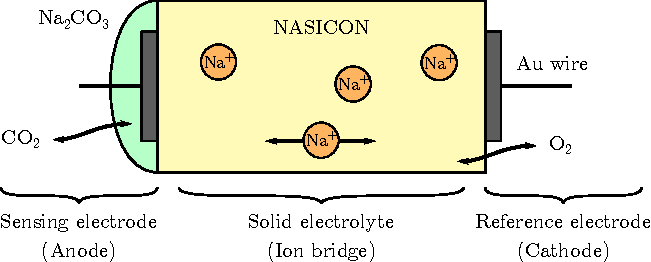
\includegraphics{1_main_matter/choos_figures/review/pot_sensor}
	\caption[Outline schematic of a potentiometric \gls{co2} sensor.]{Outline schematic of a potentiometric \gls{co2} sensor as described by Maruyama \etal{}\cite{maruyama1987}. The NASICON sandwich with one end covered in sodium carbonate makes an electrochemical cell, the electromotive force of which yields \gls{pco2}.}
	\label{fig:choos:review:pot_sens}
\end{figure}

A major improvement to the stability of potentiometric sensors has been the addition of a third reference electrode\cite{maruyama1987, kishi2007, dang2013}, or the use of a solid reference electrode instead of the above-mentioned Na$_2$O / O$_2$ interface\cite{lee2009li, lee2014, lee2015hk}. Still, even with this referencing, such sensors usually suffer from some degree of cross-sensitivity towards humidity. In addition, one of their major drawback for biomedical applications is their high operating temperature---in the 300--700{\degree}C range.

The performance of a potentiometric sensor strongly depends on the thickness of its different constituents, but also on the choice of the materials used for the electrolyte and for the sensing electrode coating. Concerning the electrodes themselves, their composition does not seem to have any significant influence on the sensing performance, since they are often made out of noble metals---such as gold\cite{maruyama1987, obata2003, kishi2007} or platinum\cite{gauthier1977, kida2001, dang2013}. The electrode wires are bound to the solid electrolyte using pastes of the same metal---possibly deposited with a stencil---which are further sintered to make an electrical bond between the solid electrolyte and the wires. For a wider contact area, the use of a gold mesh has also been proposed\cite{obata2003}. The solid electrolyte consists more often than not in NASICON, but potassium carbonate (K$_2$CO$_3$)\cite{gauthier1977}, sodium \beta-alumina\cite{liu1990}, lithium phosphate (Li$_3$PO$_4$)\cite{lee2009li, lee2014, lee2015hk}, and more recently yttrium-doped LSBO (La$_{9.66}$Si$_{5.3}$B$_{0.7}$O$_{26.14}$)\cite{ma2020} and Li$_7$La$_3$Zr$_2$O$_12$\cite{struzik2018} have also been used with some success. As for the coating of the sensing electrode, various carbonates were explored such as Na$_2$CO$_3$, Li$_2$CO$_3$ or CaCO$_3$, with similar performance. Reference materials such as yttrium stabilised zirconia\cite{maruyama1987}, BiCuVO$_x$-perovskite-oxide\cite{kishi2007}, Li$_2$TiO$_3$ / TiO$_2$\cite{lee2009li, lee2014, lee2015hk} and Bi$_8$Nb$_2$O$_{17}$\cite{dang2013} were used exhibiting good stability.

If the objective comparison of one of the above-mentioned chemicals combination with another is made difficult by the change in form-factor and film thicknesses of the reported works, one can still notice some remarkable facts. At first, in an attempt to mitigate the humidity cross-sensitivity of potentiometric sensors, the addition of barium carbonate to a lithium carbonate sensing material (BaCO$_3$ / Li$_2$CO$_3$)\cite{kishi2007, lee2009li, lee2015hk}, or the addition of lithium carbonate to an indium tin oxide sensing material (Li$_2$CO$_3$ / ITO)\cite{obata2003} have been successfully explored by several authors, yielding potentiometric sensors with no cross-sensitivity toward humidity. Then, room temperature operation of such sensors was also achieved with good sensitivity at 30{\degree}C on the 300--3000~ppm \gls{co2} range\cite{obata2003}. Finally, thin film designs were investigated yielding particularly fast---below 1~min---responding sensors\cite{choi2013, lee2014, lee2015hk}. The full range of potentiometric \gls{co2} sensors covers the 0--100\% \gls{co2} concentration.

\subsubsection{Ionic Liquids-Based Sensors}\label{subsect:choos:review:ionic_liquids}

Room temperature ionic liquids have been intensively studied since the early 2000s, with targeted applications for gas sensing and \gls{co2} sequestration in particular\cite{barrosse2010, rehman2015, behera2015, wasilewski2020}. Ionic liquids, unlike ordinary liquids, are not made out of neutral molecules but consist exclusively of ion pairs. They also exhibit a negligible vapour pressure and their electrical conductivity makes them appropriate candidates to act as liquid electrolytes. As for metal oxide sensors, the exact mechanisms underlying \gls{co2} sensing with ionic liquids are still partially unknown, although three main pathways have been proposed. One is the reduction of \gls{co2} at the anode and its further oxidation at the cathode, possibly following\cite{fapyane2020}
\begin{equation}
	\ce{CO_{2,(ads)} + e^- <=> CO^-_{2,(ads)}}
\end{equation}
although---since there is a reasonable amount of doubt about the latter equation and the existence of \ce{CO^-_{2,(ads)}}---most authors did not explicit it, or preferred the R-CO2 notation---standing for \emph{Reduced}-\gls{co2}---instead of \ce{CO^-_2}\cite{rosen2010}. \gls{co2} reduction can be measured either by a change in the impedance of the ionic liquid\cite{li2012, honda2012, ishizu2013, willa2015, willa2017}, or by amperometric or cyclic voltammetry techniques\cite{rosen2010, fapyane2020, revsbech2019}.

A second sensing scheme has been proposed, in which \gls{co2} binds with an amine to form a \gls{cil} following\cite{chen2011}:

\begin{equation}\label{eq:carbamate}
	\begin{aligned}
		\ce{RNH + CO_2 &<=> RNCOOH} \\
		\ce{RNCOOH + RNH} &\ce{<=>} \underbrace{\ce{RNH^+_2 + RNCOO^-}}_{CIL}
	\end{aligned}
\end{equation}

Since the \gls{cil} conducts electricity, it can serve as a \gls{co2} probe using different sensing schemes. Although a simple impedance measurement may be performed, Chen \etal{}\cite{chen2011} exploited the chemoluminescence of luminol in the presence of \gls{o2} instead. In their sensor, the presence of \gls{co2} in solution generated a conducting \gls{cil} as described by equation \ref{eq:carbamate}. Electric current is then passed through the \gls{cil}, reducing dissolved \ce{O_2} into \ce{O^-_2} ions which oxidises luminol. Oxidised luminol in turns emits light by chemoluminescence, which can be quantified by optical measurements.

A third sensing scheme takes advantage of the irreversible reduction of \gls{co2} into peroxydicarbonate in the presence of oxygen following\cite{buzzeo2004, xiao2013}
\begin{equation}
	\begin{aligned}
		\ce{O^{.-}_2 + CO_2 &-> CO^{. -}_4 } \\
		\ce{CO^{.-}_4 + CO_2 &-> C_2O^{. -}_6 } \\
		\ce{C_2O^{.-}_6 + O^{. -}_2 &-> C_2O^{2-}_6 + O_2}
	\end{aligned}
\end{equation}

Since it is not reversible, the latter scheme may not be used for a traditional \gls{co2} sensor, but rather for \gls{co2} detection, dosimetry or sequestration. Interestingly, this reduction of \gls{co2} in the presence of oxygen has been treated as an interference by several authors\cite{revsbech2019, fapyane2020}, who placed an oxygen trap before their \gls{co2}-sensitive ionic liquid layer to prevent it from happening. This reduction may also be the cause of the slight drift observed in some of the afore-mentioned, non-oxygen-protected sensors\cite{li2012, willa2015, willa2017}.

In most cases, ionic liquids sensors are probed by amperometric or conductimetric methods, such as cyclic voltammetry, galvanostatic or impedance measurements. However, Fabry-Perot interferometry---see Section \ref{subsect:choos:review:fibre_optic}---has also been reported\cite{wu2018} as well as acoustic resonant sensors using quartz micro-balances\cite{mineo2012, xiao2013}. The idea of such sensors is to assess the shift in frequency of a resonant element coated with an ionic liquid. When the ionic liquid adsorbs \gls{co2}, its mass increases, lowering the resonance frequency of the micro-balance. When \gls{co2} desorbs, the inverse phenomenon occurs. Of note, such acoustic resonant sensors based on \gls{co2} solubility were also explored with silicone or amine-based polymers instead of ionic liquids\cite{zhou1994, gomes1995, lee2012, hoffman2017, siefker2021}, although they often exhibit significant sensitivity to humidity.

Overall, ionic liquid sensors have been used on the physiological\cite{fapyane2020} or full 0--100\%\cite{rosen2010, mineo2012} \gls{co2} range. Response times in the 40--200~s seems reachable\cite{chen2011, mineo2012, fapyane2020} although much longer response times have also been reported, especially for \gls{co2} desorption when returning to baseline\cite{ishizu2013, willa2015, willa2017}. The accuracy of such sensors was seldom characterized, with only Chen \etal{}\cite{chen2011} mentioning a 2.05\% accuracy measured on 10 trials. The same remark holds for the sensor lifetime, reported in only one case to be over 4~months\cite{fapyane2020}. Ionic liquids sensors also exhibit a temperature-dependent response\cite{revsbech2019, fapyane2020}, and are often sensitive to \gls{co}, \gls{o2}, H$_2$, NO$_2$, N$_2$O, SO$_2$ and humidity\cite{chen2011, li2012, fapyane2020}.

%In IL :
%Buzzeo2004 : co2, IL, cycl volt + ampero
%Bruzon2017 : idem
%rehman2015 : review ILs gas sensing
% fapyane2020, rosen2010
% capone2003, rezk2020, zosel2011

\subsection{Acoustic Properties of \texorpdfstring{\gls{co2}}{CO2}}\label{subsect:choos:review:acoustic}

\subsubsection{Time of Flight Acoustic Sensors}\label{subsect:choos:review:tof}

% Speed of sound in gases : sqrt(gamma*R*T_k/M)
% R = 8314, cf sound_speed.py
Time of flight sensors are based on the difference in sound velocity between \gls{co2} and other gases---\eg{} 351, 330 and 269~m.s$^{-1}$ for \gls{n2}, \gls{o2} and \gls{co2} under 1~atm and 25{\degree}C, respectively\cite{giacobbe1993}. Thus, a simple time of flight sensor can be constructed for \gls{co2} sensing, consisting in an ultrasound emitter and receiver pair, facing each other in the analyte gas mixture. Joos \etal{}\cite{joos1993}, for instance, performed acoustic measurements using a 20~cm tube at the end of which the ultrasound transducers were attached. The authors were able to measure the \gls{co2} content of a \gls{co2} / \gls{n2} gas mixture on the full 0--100\% \gls{co2} range with an accuracy of 0.3\%. An outline schematic representing the working principle of their experiment is depicted in Figure \ref{fig:choos:review:time_of_flight}.

\begin{figure}
	\centering
	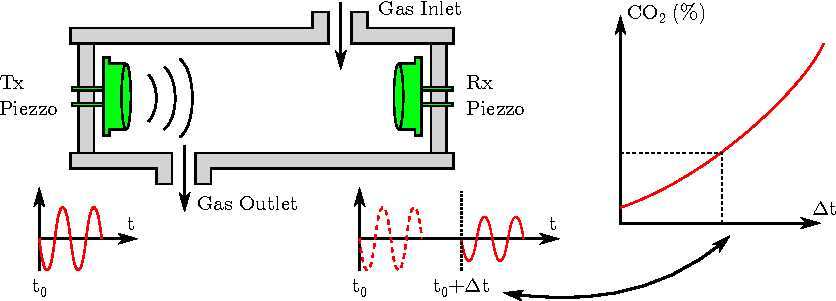
\includegraphics{1_main_matter/choos_figures/review/time_of_flight}
	\caption[Outline schematic of a time of flight \gls{co2} sensor.]{Outline schematic of a time of flight \gls{co2} sensor as described by Joos \etal{}\cite{joos1993}. Two ultrasound (40~kHz) transducers---emitter (Tx) and receiver (Rx)---are placed at both ends of an acoustic chamber which may consist of a simple tube. A burst of ultrasound is emitted at $t_0$ (on the left) and arrives at $t_0+{\Delta}t$ at the receiver (on the right). The ${\Delta}t$ value can then yield the percentage of \gls{co2} in the gas mixture using velocity-based calculations.}
	\label{fig:choos:review:time_of_flight}
\end{figure}

These sensors usually have long path lengths---20~cm in the above-mentioned work\cite{joos1993}---which may be difficult to embed in a portable apparatus. Still, they can provide low latency measurements, since their response time is only limited by the time taken by the analyte gas mixture to fill the acoustic chamber. Interestingly, recent research by Cicek \etal{}\cite{cicek2019} demonstrates another exploitation of the difference in sound velocity between \gls{n2} and \gls{co2}, using an array of miniature Helmholtz resonators, whose resonance frequency shifts depending on the \gls{co2} concentration to which they are exposed. They achieved \gls{co2} sensing in the 0--1\% range with a 70~mm radius sensing array.

However, while this technique may seem interesting at first glance for its low cost and long-term stability, it is usually limited to a mixture of two gases\cite{gerlach2019_ch9}. Consequently, it might be unusable in the context of biomedical \gls{co2} monitoring. Indeed, most human tissues not only produces \gls{co2} and consumes \gls{o2}, but also evaporates water. As such, a gaseous volume equilibrated with human tissues may contain as many as four different gases---\gls{co2}, \gls{o2}, \gls{n2} and \gls{h2o}---whose amounts cannot be found with a single pulse velocity measurement.

\subsubsection{Acoustic Attenuation Sensors}\label{subsect:choos:review:acoust_att}

The acoustic attenuation sensing scheme is based on the phenomenon of vibrational relaxation, which consists in the reduction in intensity of a propagating acoustic wave in a gas. This attenuation depends on the sound frequency and the specific gas or gas mixture in which it occurs\cite{evans1972, bass1990}. Acoustic attenuation measurements performed at different frequencies allows to establish the acoustical absorption spectrum---i.e. attenuation intensity as a function of the acoustic wave frequency---of a gas mixture. Several such spectra are presented in Figure~\ref{fig:choos:review:sound_att}, and can be used to identify the different gases that compose an analyte gas mixture as well as their proportion in the latter. To do so, an apparatus similar to that presented in Figure~\ref{fig:choos:review:time_of_flight} may be used, but with multiple emitter / receiver pairs placed at different distances. Then, measurements of the sound attenuation and velocity can be performed, yielding an absorption value. The latter may in turn be compared with theoretical calculations---or experimental data---for a \gls{co2} / \gls{n2} gas mixture, leading to a \gls{pco2} value.

\begin{figure}
	\centering
	\includegraphics{1_main_matter/choos_figures/review/tikz/out/petculescu}
	\caption[Acoustical absorption spectra of diverse nitrogen mixtures.]{Acoustical absorption spectra of diverse nitrogen mixtures. Data source: Petculescu \etal\cite{petculescu2006a}.}
	\label{fig:choos:review:sound_att}
\end{figure}

Theoretical and practical applications of this phenomenon are available in the literature\cite{dain2001, cottet2004, ejakov2003, petculescu2006a, petculescu2006b, jia2018}. However, at least to the best of our knowledge, vibrational relaxation applied to \gls{co2} sensing never went further than the proof of concept presented by Petculescu \etal{}\cite{petculescu2006b}. Unlike most of the other sensors presented in this review, cross-sensitivity towards \gls{o2} should be negligible. Indeed, \gls{o2} does not exhibit any vibrational relaxation phenomenon in the 10$^3$--10$^7$~Hz.atm$^{-1}$ range\cite{ejakov2003}. The influence of humidity may be another source of concern, however. If the lower mode of water vibrational relaxation occurs at much lower frequencies than that of \gls{co2}\cite{zuckerwar1981}, higher frequencies components are also present at high humidity fraction which can interfere with \gls{co2} measurements\cite{ejakov2003}. In addition, temperature should be measured and compensated for, as it influences sound propagation, and thus the position and amplitude of the acoustical absorption peaks\cite{dain2001}.

\subsection{Comparison Table}\label{subsect:choos:review:comp_table}

Although an objective comparison of the above-mentioned \gls{co2} measurement techniques is made exceedingly difficult due to the incompleteness of most of the referenced works, we tried to do our best to gather state of the art performance for the different sensing schemes presented. The pith and marrow of our literature review is thus summarised in Table \ref{tab:choos:review:resume_techniques}.

We gently warn the reader that each column of the table contains the best performance reported in the literature for a given criterion and that no sensor may exist with all the characteristic presented in a given row. For instance, concerning ionic liquids-based sensors, Chen \etal{}\cite{chen2011} reported a 2.05\% accuracy but with a 2~min response time, while Mineo \etal{}\cite{mineo2012} reported a 40~s response time without reporting the accuracy of their sensor. Still the \enquote{ionic liquid} row of Table \ref{tab:choos:review:resume_techniques} contains both the 2.05\% accuracy and 40~s response time, even if no sensor exists with such characteristics.

Finally, although most criteria are self-explanatory, a few additional comments may be necessary for a sound understanding and interpretation of this table. First, the lifetimes of several sensor families---and especially that of the (photo-)acoustical ones---are not explicitly reported in the literature. Yet, since \gls{ndir} sensors were reported to reach a lifetime of at least 15~years\cite{gibson2013}, and since acoustical building blocks---\eg{} ultrasonic transducers---usually last for years, the infinity symbol ($\infty$) was used, meaning that a lifetime of at least several years should be expected. Second, the calibration need refers to the need to re-calibrate a sensor frequently---\ie{} every few hours or days---due to the presence of a significant drift in its response. This criterion does \emph{not} refer to the initial sensor calibration that may be performed in the factory. Third, the response time of the evaluated sensors was often measured using test benches which flush the sensors with a continuous flow of a gas mixture containing a known \gls{co2} concentration. In such a configuration, the four sensors noted with an $(a)$ are supposed to respond as soon as the latter gas mixture flows inside their embodiment, hence the $\leq 1$~s indication. In practice, however, the response time strongly depends on the sensor housing dimensions, since \gls{co2} will have to diffuse from the analyte gas---or medium---inside the sensor embodiment.

\afterpage{
\begin{landscape}
\def\arraystretch{1.25}
\begin{table}
	\centering
	\begin{adjustbox}{center}
	\begin{tabular}{c|c|c|c|c|c|c|c}
		\specialcell{Criterion $\rightarrow$\\$\downarrow$ Technique} & Lifetime & \specialcell{Calibration\\need} & \specialcell{Humidity cross-\\sensitivity} & Accuracy & \specialcell{Response\\time} & \specialcell{Miniaturisation\\potential} & References \\ \hline \hline
		
		\specialcell{\gls{ndir}\\(Section \ref{subsect:choos:review:ndir})} & $\geq15$~years & No & No & 0.03\% & $\leq$1~s $^{(a)}$ & \specialcell{Moderate (down to\\$10\times 10\times 0.5$~mm$^3$)} & \cite{zhang2010, gibson2013, jing2020, popa2019}\\ \hline
		% 15 years: gibson, 0.03%: zhang, 1sec: gibson, dims: jing2020
		
		\specialcell{Photoacous.\\(Section \ref{subsect:choos:review:photoacous})} & ? ($\infty$) & No & No & 1\% & $\leq$1~s $^{(a)}$ & Low ($\sim$cm) & \cite{kosterev2006, scholz2017, eberl2019} \\ \hline
		
		\specialcell{Wet Conduct.\\(Section \ref{subsect:choos:review:wet_conduct})}& ? & \specialcell{Yes\\ (0.4\% drift / hour)} & Yes (dries out) & ? & 5~s & \specialcell{High (down to\\100~\textmu{}m thickness)} & \cite{varlan1997, mirtaheri2004b} \\ \hline
		
		\specialcell{S-S elec.\\(Section \ref{subsect:choos:review:ssel})} & 80 days & Yes (0.03~mV/h) & Yes (dries out) & 0.03\% (0--100~mmHg) & 30~s & \specialcell{High (down to\\10~\textmu{}m thickness)} & \cite{severinghaus1958, hahn1980, shin2000, beyenal2004} \\ \hline
		
		\specialcell{\gls{isfet}\\(Section \ref{subsect:choos:review:isfet})} & $\geq$ 30 days & Yes (0.23~mV/h) & Yes & ? & 60~s & \specialcell{High (down to\\100~\textmu{}m thickness)} & \cite{hu1989, hsieh2014} \\ \hline
		
		\specialcell{Dye-based\\(Section \ref{subsect:choos:review:dye_based})} & 19~months & No & Yes & 0.1\% & $\leq1$~s & \specialcell{Excellent (down to\\1~\textmu{}m thickness)} & \specialcell{\cite{mills1997, mills2009, dansby2010, atamanchuk2014}\\\cite{fernandezramos2018, fernandezramos2019}} \\ \hline
		% 19 months: fernandezramos2019, 0.1%: fernandezramos2018, <1sec: mills1997, calibration need: ge2014, atamanchuk2014, mills2009 pour info générales
		
		\specialcell{Optical fiber\\(Section \ref{subsect:choos:review:fibre_optic})} & ? & ? & Yes & 4.1\% & 40--75~s & \specialcell{Excellent (down to 55~nm\\coating thickness)} & \cite{melo2014, chong2015, hromadka2018}\\ \hline
		% 4.1%: melo2014, 40--75s: chong2015, 55nm: hromadka2018
		
		\specialcell{Metal Oxide Ads.\\(Section \ref{subsect:choos:review:metal_oxide})} & $\geq$5~months & No & Yes (low) & 1.6\% & 30~s & \specialcell{Excellent (down to\\ 125~nm thickness)} & \specialcell{\cite{ishihara1993, mizuno1993, ishihara1995, haeusler1996}\\ \cite{herran2009, jeong2016, joshi2020}}\\ \hline
		
		\specialcell{Graphene\\(Section \ref{subsect:choos:review:graphene})} & $\geq$90~days & No & Yes & 0.8\% & 3~s & \specialcell{Excellent (down to\\ 3~nm thickness)} & \cite{yoon2011, shaban2019, akhter2021}\\ \hline
		
		\specialcell{Electro. Cells\\(Section \ref{subsect:choos:review:electrochem_cell})} & $\geq$2~years & No & No & 4\% & 2--4~s & \specialcell{Excellent (down to\\1~\textmu{}m thickness)} & \cite{kaneyasu2000, lee2009li, choi2013, lee2014}\\ \hline
		
		\specialcell{Ionic liquids\\(Section \ref{subsect:choos:review:ionic_liquids})} & $\geq$4~months & No & No & 2.05\% & 40~s & \specialcell{Excellent (down to\\ 430~nm thickness)} & \specialcell{\cite{chen2011, mineo2012, willa2015}\\ \cite{revsbech2019, fapyane2020}}\\ \hline
		
		\specialcell{Time of flight\\(Section \ref{subsect:choos:review:tof})} & ? ($\infty$) & No & Yes (low) & \specialcell{0.3\%\\ (0--10\% range)} & $\leq$1~s $^{(a)}$ & Low ($\sim$cm) & \cite{joos1993} \\ \hline
		
		\specialcell{Acous. Att.\\(Section \ref{subsect:choos:review:acoust_att})} & ? ($\infty$) & No & ? & ? & $\leq$1~s $^{(a)}$ & Low ($\sim$cm) & \cite{petculescu2006a, petculescu2006b}
		% humidity cross-sens: ? depend frequence...
		
	\end{tabular}
	\end{adjustbox}
	\caption[An overview of the presented \gls{co2} sensing techniques.]{An overview of the presented \gls{co2} sensing techniques. ($\infty$): expected to be at least several years. $(a)$: limited primarily by the diffusion of the analyte gas inside the enclosure of the sensor. Please refer to detailed explanations in Section \ref{subsect:choos:review:comp_table}.}
	\label{tab:choos:review:resume_techniques}
\end{table}
\end{landscape}
}

\section{Potential Application to Transcutaneous Sensing}\label{sect:choos:techno_choice}

Returning to the development of next-generation \gls{ptco2} sensors, let us briefly review past attempts before choosing one of the \gls{co2} sensing techniques mentioned above, based on the specificities of transcutaneous \gls{co2} sensing.

\subsection{Past Attempts}\label{subsect:choos:pot:past_attempts}

The \ssel{} appeared in the late 1950s, underwent only minor improvements since then, and reigns supreme over the \gls{ptco2} monitoring market\cite{severinghaus1986_3, mari2019}. Yet, several authors have been trying to push forward other means of measuring a subject's \gls{ptco2}, mainly using \gls{ndir} sensing and mass spectroscopy, as disclosed in the following sections. It is also worth mentioning here that we measured the absorption spectrum of \gls{co2hb} while searching for a non-invasive alternative to \gls{ptco2} monitoring, even if this track proved to be but a dead end, as \gls{co2hb} and \gls{hb} have identical absorption spectra---see Section~\ref{sect:co2hb:pulse_carbametry}.

\subsubsection{Non-Dispersive Infrared and Transcutaneous Sensing}

Regarding \gls{ndir}, a couple of works by Eletr, Greenspan \etal{} surfaced in the early 1980s\cite{eletr1978, greenspan1981}, describing a Hewlett-Packard capnometer that collects the \gls{co2} exhaled by the skin inside a small sampling chamber probed by infrared radiations. Despite the fair performances achieved---up to 48~h of continuous monitoring, an SD of 0.2~kPa (1.5~mmHg) between \gls{paco2} and \gls{ptco2} on 3--6~h sessions and a response time about 90~s\cite{eletr1978}---the main drawback of this sensor was the need to strip the stratum corneum with 20--50 successive applications of adhesive tape so as to reach a reasonable response time.

The \gls{ndir} track was then dropped until the mid 2010s and the advent of rate-based approaches by the team of Chatterjee, Ge, Iitani \etal{}\cite{chatterjee2014, chatterjee2015, ge2018, iitani2021} at first and by the team of Grangeat \etal{}\cite{grangeat2019, grangeat2020} in a second move. If the latter work is insufficiently detailed---especially the explanations concerning the sensing part itself---the former allows for a sound understanding of the rate-based approach. This approach consists in placing a sampling cup against the skin to collect transcutaneously exhaled \gls{co2}, but---contrary to what was done in the earlier work of Eletr, Greenspan \etal{}---no time is left for the gas in the cup to reach an equilibrium with the skin \gls{co2} content. Rather, the gas in the cup is flushed with fresh air or pure \gls{n2}, and its \gls{co2} fraction is then measured using a conventional \gls{ndir} sensor. Theoretically, the so-obtained \gls{co2} diffusion rate is only function of \emph{(i)} the patient's \gls{ptco2} and \emph{(ii)} their skin diffusivity towards \gls{co2}\cite{chatterjee2015}. However, since this latter parameter is not known accurately and fluctuates a lot depending on the skin temperature\cite{shaw1930, scheuplein1976}, measurement site\cite{adamczyk1966, levshankov1983} and subject at hand\cite{ernstene1932a}, the rate-based approach is most likely limited to trend analysis at best\footnote{In addition to the presented references, the mnemonist reader surely recalls the large variability of measured skin \gls{co2} conductivities reported in Section~\ref{sect:tcco2:frontiers_article}.}.

In the afore-mentioned works, it should also be noted that contrary to the teams of Chatterjee, Ge, Iitani, \etal{}, those of Grangeat, Eletr, Greenspan \etal{} heated the skin in the 35--43{\degree}C range, likely so as to boost the skin conductivity towards \gls{co2}, as explained in Section~\ref{sect:tcco2:frontiers_article}.

\subsubsection{Mass Spectroscopy and Transcutaneous Sensing}

Overcoming the issue of the latter rate-based approach, a more sophisticated technique has been explored in parallel by Mc Ilroy's team in the early 1980s\cite{mcilroy1978, hansen1980, targett1984}, using mass spectrometry for \gls{co2} detection. The main idea behind their work is to perform a per-subject and per-site calibration to first determine the skin permeability towards \gls{co2} and only then access to the patient's \gls{ptco2}. While in its first version, their sensor required a change of membrane to perform this calibration\cite{hansen1980}, a second version with two sampling chambers and an additional valve solved this need for external intervention\cite{targett1984}. In their setup, the skin was also stripped with 5--10 applications of adhesive tape beforehand, and heated to 43--45{\degree}C. They achieved a correlation factor of 0.81 between \gls{paco2} and \gls{ptco2}, and a response time below 5~min. The main drawback of their technique is of course the need for a mass spectrometer, which is bulky, requires maintenance, and costs tens if not hundreds of thousands of euros. Their dual-rate technique, however, might presumably be adapted to a \gls{ndir} sensing scheme, thus compensating for the fluctuations of skin diffusivity mentioned in the previous section, and emphasised in our above-presented clinical study---Section~\ref{sect:tcco2:frontiers_article}.

\subsection{Transcutaneous Sensing Constraints}

An effective biomedical \gls{ptco2} sensor should fulfil two main objectives: it must respond swiftly to a patient's haemodynamic changes, and it must measure a \gls{ptco2} that reflects accurately their state. To do so, the sensor design must take into account the two main characteristics of \gls{co2} diffusion through the skin, which both are temperature-dependent:

\begin{enumerate}
	\item[--] The correlation between the \gls{pco2} measured at the skin surface---that is \gls{ptco2}---and that of arterial blood---that is \gls{paco2}. This correlation will determine the ability of the sensor to give clues about the patient's status through a \gls{ptco2} reading, it was briefly mentioned in Section~\ref{subsect:tcco2:frontiers:acc_impact} and is further detailed below.
	\item[--] The exhalation rate of \gls{co2} through the skin into the sensor, which will determine the response time of the sensor. This aspect was already covered in great details in Section~\ref{sect:tcco2:frontiers_article} and will not be discussed any further.
\end{enumerate}

Additionally, the sensor design must also take into account the specificities of cutaneous sensing---\ie{} temperature, humidity, acidity, and \gls{o2} presence---outlined in Section~\ref{sect:tcco2:skin_conditions}.

\subsubsection{Correlation Between \texorpdfstring{\gls{paco2}}{paCO2} and \texorpdfstring{\gls{ptco2}}{tcpCO2}}\label{subsect:choos:techno_choice:correl_pa_ptc}

The \gls{paco2} / \gls{ptco2} correlation has been demonstrated at 42{\degree}C and above\cite{conway2018}, but heating the skin is not only uncomfortable for the patient but also energy consuming---which limits the ability of the sensor to be integrated into a wearable, battery-powered device---and potentially harmful due to risk of thermal injury, especially above 44{\degree}C---see Appendix~\ref{annsect:temp_harm} for a more detailed discussion on this topic.

For these reasons, working at low skin temperature seems highly desirable. To the best of our knowledge, only the work of Wimberley \etal{}\cite{wimberley1985a} studied the influence of skin temperature on the correlation between \gls{paco2}---through arterialised capillary blood, to be accurate---and \gls{ptco2}. Their study covers the full 37--45{\degree}C range and they show a fair---$r=0.93$---correlation between capillary and transcutaneous \gls{pco2}, even at a temperature as low as 37{\degree}C. Yet, \mfrin{}further research on the topic would be valuable since other sources argue that a higher probe temperature still yields narrower limits of agreement for \gls{ptco2}\cite{conway2018}.

\subsection{Recommendations for a Closed-Chamber Design}

Summarising the above, the following parameters should be carefully taken into account when designing a next-generation \gls{ptco2} sensor using a closed-chamber---\aka{} equilibrium-based---design:
\begin{enumerate}
	\item \textbf{The skin temperature} influences both the sensor \emph{response time} through the \gls{co2} rate of diffusion and its \emph{accuracy} through the \gls{paco2} / \gls{ptco2} correlation. The clinical study presented in Section~\ref{sect:tcco2:frontiers_article} revealed that a skin temperature in the 35--38{\degree}C range should yield a reasonably fast sensor---only 35\% slower than when using a 44{\degree}C skin temperature. Accuracy-wise, despite a lack of data in the literature, the latter study also tends to indicate that heating the skin in the afore-mentioned range could be enough to yield a clinically-usable \gls{ptco2} reading.
	\item \textbf{The form factor of the sensor} directly influences its response time. The analyses presented in Section~\ref{sect:tcco2:response_time} revealed that a volume to surface ratio of 100~\textmu{}m or below is required to yield response times below 10~min.
	\item \textbf{The cutaneous measuring conditions} may hamper the adequate functioning of the sensor. More specifically, Section~\ref{sect:tcco2:skin_conditions} revealed that the skin is a highly hypoxic medium, from which numerous acidic compounds may emanate, and which exhibits saturating humidity levels when occluded.
\end{enumerate}
The \gls{co2} sensing techniques presented in Section~\ref{sect:choos:sensors_review} are reviewed below according to these latter aspects.

At first, only some of them can deal with a height limitation of only 100~\textmu{}m. In that respect, \gls{ndir}, photoacoustic, time-of-flight and acoustic attenuation sensors cannot be miniaturised to reach such a thickness. Second, the use of metal oxide thin films as well as electrochemical cells should be highly discouraged since both operate at several hundreds degrees Celsius. As such, using them close to the skin may entail a significant safety hazard. Then, conductometric and \gls{isfet}-based sensor as well as the \ssel{} all suffer from important drift issues, making them unusable for more than a few hours, or days. Optical fiber-based sensors, for their part, require an expensive and bulky measurement apparatus which seems hardly embeddable into a wearable device.

Remain the ionic liquid-, graphene- and dye-based sensors. While recent research on ionic liquid-based sensors showed definite progress, they are still extremely sensitive to \gls{o2} and often exhibit particularly elevated recovery times\cite{willa2017, fapyane2020}. Similarly, recent developments pave the way for graphene-based \gls{co2} sensors\cite{akhter2021}, but their important cross-sensitivity towards humidity precludes their use without an additional humidity sensor for referencing, due to the skin humidity. Thus, the option of choice appears to be the more mature dry dye-based sensors for they can yield thin enough, fast responding, and long lasting \gls{pco2} sensors---see Section \ref{subsect:choos:review:dye_based}. In addition, dye-based sensors can be dissociated into a \gls{co2} sensing part on the one hand, and an optical probing part on the other hand, as presented in Figure \ref{fig:choos:pot:fluo_patch}. This design is especially interesting since it makes possible to use a disposable sensing patch that can be replaced every few days while the sensing head can be reused indefinitely. Finally, the multilayer structure of the patch seems well adapted to existing manufacturing processes---roll-to-roll in particular---for mass production\cite{briand2011, kostler2011}.

\begin{figure}
	\centering
	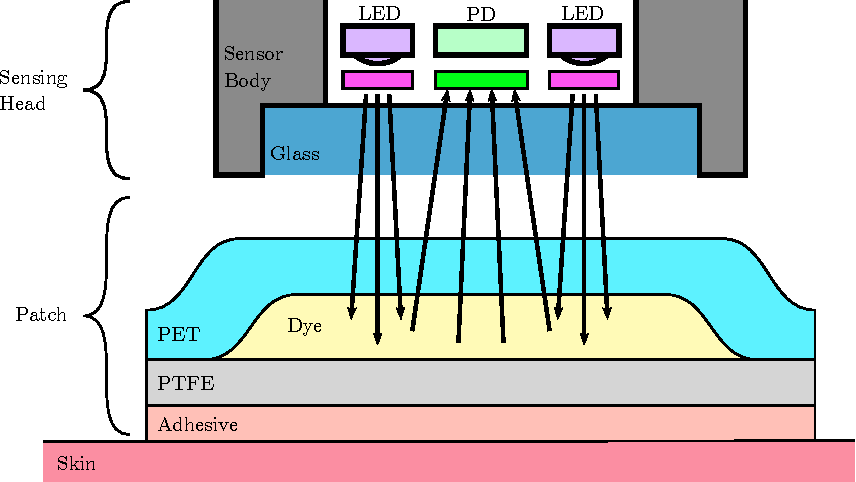
\includegraphics{1_main_matter/choos_figures/review/fluo_patch}
	\caption[Schematic outline of a dye-based fluorescent transcutaneous sensor, consisting in two parts.]{Schematic outline of a dye-based fluorescent transcutaneous sensor, consisting in two parts. \textbf{Top:} a sensing head with the \glspl{led} and photodiode covered with their emission and reception filters (bright purple and green rectangles) and enclosed in a solid body, protected by a covering glass. \textbf{Bottom:} a multilayer sensing patch stuck on the skin, consisting in---from top to bottom---a transparent layer, impermeable towards \gls{co2}---\eg{} \gls{pet}---a layer of \gls{co2} sensitive dye in a polymer matrix, a layer of ion-impermeable, \gls{co2}-permeable material such as \gls{ptfe} for \gls{co2} diffusion from the skin into the dye, and a thin adhesive layer to maintain the patch onto the skin. See Section \ref{subsect:choos:review:dye_based} for a detailed review of material choices as well as their advantages and drawback when designing a dye-based \gls{co2} sensor.}
	\label{fig:choos:pot:fluo_patch}
\end{figure}

\subsection{Other Perspectives}

Apart from a closed-chamber design---for which dye-based sensing seems to be the most appropriate sensing technique---transcutaneous \gls{co2} monitoring may also be envisioned using a rate-based approach, or \gls{drs}.

\subsubsection{Rate-Based Approach}\label{subsect:choos:pot:rate_based}

The rate-based approach has already been presented in Section \ref{subsect:choos:pot:past_attempts}, and corresponding theoretical developments can be found in the work of Chatterjee \etal{}\cite{chatterjee2015}. The main advantage of this approach is that it relaxes the form factor constraint highlighted above in the closed-chamber case. Thus, \gls{ndir} sensing can be used instead of a dye-based thin film, with better lifetime, accuracy, and selectivity over the latter. These advantages made \gls{ndir} sensing the foremost choice of the authors who considered using a rate-based approach for transcutaneous \gls{co2} sensing\cite{chatterjee2014, chatterjee2015, ge2018, grangeat2019, grangeat2020}.

The biggest issue with this approach is the large inter-subject variability in skin diffusivity values towards \gls{co2}. Indeed, all studies that reported measurements of the cutaneous \gls{co2} exhalation rate do mention this variability---see Table~\ref{table:tcco2:diff_rate_lit}---and factors in the 1.5--2 range are not unheard of, between the exhalation rates of two individuals, even at the same skin site and temperature. Our own investigations revealed even wider variabilities, with maximum-minimum ratios in the 2.8--9.2 range for a given skin site / temperature pair---see Table~\ref{table:tcco2:qs_values}. This strong variability among individuals precludes the measurement of \emph{absolute} \gls{ptco2} by means of a rate-based approach without further improvements of the technique. This was recently demonstrated by several authors, who could only report trend analyses of skin \gls{co2} exhalation rate, and no rate-based absolute \gls{ptco2} readings\cite{ge2018, grangeat2019, grangeat2020}. Further still, the recent work of Iitani \etal{}\cite{iitani2021} clearly illustrates the afore-mentioned inter-subject variability with a factor of more than ten between the exhalation rates of two subjects (S2 and S6 on their Figure 4-H). An exception may exist for neonates, however, whose exceedingly thin skin could be more homogeneous than that of adults, resulting in less variability in their skin \gls{co2} exhalation rate. This latter \emph{hypothesis} might explain why Chatterjee \etal{}\cite{chatterjee2015} were able to demonstrate a significant correlation between skin \gls{co2} exhalation rate and \gls{ptco2} in 4 preterm neonates with gestational ages ranging from 23 to 36 weeks.

\mfrin{}To overcome this challenge, several tracks can be followed. At first, further studies on the \gls{co2} exhalation phenomenon through human skin would be welcome. As already mentioned, the currently available literature on this topic is ageing, and rarely includes more than a handful of subjects. In addition, the temperature dependence of the exhalation rate also needs to be carefully studied by regulating the skin temperature, and not that of the ambient air surrounding it. A better understanding of the process of \gls{co2} diffusion through the skin and of the different variables influencing the said process may help to better characterise---and perhaps even compensate for---the intra- and inter-subject variations in \gls{co2} exhalation rate with skin site, skin temperature, or time of the day. In this aspect however, the clinical study presented in Section~\ref{sect:tcco2:frontiers_article} gives little clue---if not little hope---only confirming the wide variability mentioned above.

Second, dual membrane techniques---such as that presented by Targett \etal{}\cite{targett1984}---may be adapted to modern sensing techniques in a setup and compactness close to that of Grangeat \etal{}\cite{grangeat2019} prototype, using two different sensing channels, for instance.

Third, the need for an absolute \gls{ptco2} reading could also be mitigated in two ways. First off, by mean of a punctual per-subject calibration, following the example of non-invasive, cuffless, \gls{ppg}-based, arterial blood pressure measurements\cite{xing2019, shao2020}. In this sensing scheme, the actual \gls{ptco2} could be measured from time to time using a reference \gls{ptco2} monitor, whose measurements would then serve to calibrate a lighter, wearable, rate-based device. This would allow to share a main---expensive---\gls{ptco2} monitor among multiple patients, in a clinical setting. Alternatively, it could also be envisioned that rate-based devices do not provide any absolute \gls{ptco2} reading. Rather, they may provide the user with trend analysis only, raising alarms following the crossing of certain thresholds or abrupt variations. This last approach, however, may be difficult to introduce into medical practice without further clinical studies, even though the clinical interest of similar variability metrics for other physiological variables---such as heart rate\cite{kim2018} or oxygen saturation\cite{moret2014, clarke2016}---is encouraging in this regard.

\subsubsection{\texorpdfstring{\glsfirst{drs}}{DRS}}\label{subsect:choos:pot:drs}

As stated in Section \ref{subsect:choos:review:ndir}, dissolved \gls{co2} measurements can be performed not only in the gaseous phase, but also in aqueous solution\cite{schaden2004}. This result was also demonstrated for whole blood samples, the \gls{pco2} of which could be retrieved with a standard error of about 5~mmHg, using infrared spectroscopy in the 1024--2290~nm range\cite{domjan1994}. Further still, it has been recently suggested in a patent that transcutaneous \gls{co2} measurements could be performed using mid-infrared \glspl{led} of wavelength \enquote{between about 2~\textmu{}m and about 18~\textmu{}m}\cite{marasco2020}. Although patents do not constitute scientific evidence\cite{freilich2019}, the idea has been put forth, and \mfrin{}further research would be interesting on the topic, in order to assess the feasibility of such transcutaneous \gls{co2} measurements. \emph{Prima facie}, two major challenges conceivably need to be solved for \gls{drs}-based transcutaneous measurements.

First, contrary to pulse oximetry, the possibility to measure a pulsatile absorbance component due to \gls{co2} dissolved in the arterial blood by transcutaneous \gls{drs} probing in the mid-infrared is vastly unknown. If possible though, the whole theoretical background developed over the years for pulse oximetry and \gls{ppg} signal processing\cite{tamura2019} could be translated to \gls{co2} measurements.

Second, the penetration depth of mid-infrared light in the human tissues may also be a source of concern, especially because of the elevated infrared absorbance of water. Indeed, water absorbance becomes predominant in the tissues in the near and mid infrared\cite{jacques2013}, with values over 1~cm$^{-1}$ above 1150~nm, and over 5~cm$^{-1}$ above 1380~nm\cite{kou1993}. This may cause serious difficulties for mid-infrared tissue probing and lead to a very low signal to noise ratio, which may be the reason why Marasco \etal{} suggest the use of a lock-in amplifier for transcutaneous \gls{co2} measurement in their patent\cite{marasco2020}.

In both cases, heating the skin to provoke a local hyperaemia---as mentioned in Section \ref{subsect:tcco2:subcut_bf}---may tackle the above-mentioned probing depth issue, by bringing the \gls{co2} content of subcutaneous tissues close to that of arterial blood.

\subsection{Synthesis}

\gls{ptco2} is the least invasive and the most accessible proxy for \gls{paco2}---which is of major clinical significance---given that the skin temperature is at least above 37{\degree}C (Section \ref{subsect:tcco2:frontiers:acc_impact}). \gls{ptco2} may be measured by two means: either exploiting the cutaneous respiration phenomenon, or by direct infrared tissue probing, using \gls{drs}.

While the feasibility of the latter technique has yet to be demonstrated for \emph{in vivo} transcutaneous \gls{co2} monitoring, it seems like an appetising proposal (Section \ref{subsect:choos:pot:drs}). Indeed, it would require merely a mid-infrared source and detector---which are readily available components, see Section \ref{subsect:choos:review:ndir}---and conceivably the same kind of electronic as that already embedded in commercially available pulse oximeters. Yet, such an application of \gls{drs} remains vastly hypothetical at the time of writing this review, and \mfrin{}further research would be needed on the topic, so as to consolidate the above-mentioned research works.

Cutaneous respiration, on its part, has long proven to be a reliable access route to \gls{ptco2}, by capturing the \gls{co2} exhaled by the skin inside the embodiment of a \gls{co2} sensor (Section \ref{subsect:choos:review:ssel}). A simple model for such a closed-chamber sensor design has been extensively described, as well as its expected response time as a function of its form factor (Section \ref{sect:tcco2:response_time}). We conclude that, in such a closed-chamber design, the compactness of the \gls{co2} sensor is crucial in order to reach reasonable response times. Taking into account other merit criteria such as response time, long-term stability and accuracy, \textbf{we put forth the application of dye-based \gls{co2} sensing to serve such a purpose}.

Alternatively, a rate-based approach may be envisioned using a constant flow of air or N$_2$ passing over the skin, and being analysed thereafter (Section \ref{subsect:choos:pot:rate_based}). The main advantage of this technique is that the form factor of the sensor itself is not as much a source of concern as in the closed-chamber setup. Thus, other sensing techniques can be envisioned such as \gls{ndir} \gls{co2} sensing. However, several challenges remain, precluding rate-based approaches to yield an absolute \gls{ptco2} measurement. In particular, a better characterisation of human skin \gls{co2} exhalation rate, dual membrane approaches, or self-calibration from time to time are all interesting leads that need further exploration.

\section{Dye-Based \texorpdfstring{\gls{co2}}{CO2} Sensing}\label{sect:choos:dye_based}

Hopefully, the reader now has a satisfactory understanding of the ins and outs of transcutaneous \gls{co2} measurement: why \gls{ptco2} is clinically important---Chapters~\ref{chap:intro} and \ref{chap:co2hb}---what are the specificities of transcutaneous \gls{co2} sensing---Chapter~\ref{chap:tcco2}---and what \gls{co2} sensing technique best fits these specificities---firs half of the present chapter. \textbf{The remainder of this doctoral work focuses solely on the intricacies of dye-based \gls{co2} sensing.} While Chapter~\ref{chap:thin_film} details the \emph{practical realisation} of \gls{co2}-sensing fluorescent thin film---\ie{} what encapsulating strategy, polymer, and fluorophores were chosen, what concentrations were actually used, and what response towards \gls{co2} was achieved, also giving insights on the optoelectronics setup that was used---the second half of the present chapter is devoted to the \emph{theoretical foundations} of dye-based \gls{co2} sensing. More specifically:
\begin{itemize}
	\item[--] The chemistry of wet and dry sensors is given in Section~\ref{sect:choos:dye_based:chemistry}.
	\item[--] The available optical measurement schemes and the associated signal processing techniques are presented in Section~\ref{sect:choos:dye_based:optical_schemes}.
	\item[--] The \gls{dlr} sensing scheme, which has been chosen among the latter schemes to fulfil the goal of this doctoral work, is then further detailed in Section~\ref{sect:choos:dye_based:dlr_theory}.
\end{itemize}

\subsection{Sensing Chemistry}\label{sect:choos:dye_based:chemistry}

The development of dye-based \gls{co2} sensors occurred in two main phases, corresponding to the afore-mentioned \emph{wet} and \emph{dry} sensor families---see Section~\ref{subsect:choos:review:dye_based}. Briefly, a first line of works emerged in the mid eighties introducing wet-type sensors\cite{vurek1983, zhujun1984a, zhujun1984b, opitz1984}, which underwent no major changes for several years until the pivotal works of Andrew Mills in the early nineties, who introduced dry-type sensors in a series of seminal papers\cite{mills1992, mills1993, mills1997}. The main difference between wet and dry sensors is the following. In wet sensors, the \gls{co2}-sensitive pigment is dissolved in an aqueous solution, which makes water molecules directly available for the hydration and dissociation of \gls{co2} into bicarbonate ion and protons. On the contrary, in dry sensors, all chemicals are entrapped inside a solid polymer layer. Since hydration water is no longer present, additional chemicals---termed phase transfer agents---are added whose role is to bind water molecules to make them available for the afore-mentioned dissociation. The differences and common points between these two modalities will become more evident in the next subsections.

\subsubsection{Wet Sensors}

\paragraph{The \texorpdfstring{\pH-\gls{pco2}}{pH-pCO2} Relationship}\mbox{}\\

Let us consider a solution of sodium bicarbonate in water, equilibrated with a gas mixture with a \gls{co2} partial pressure \gls{pco2}. The following equilibria take place in the solution\cite{jensen1979, mills2009}:
% Dirty as hell, but working
% https://tex.stackexchange.com/questions/96568/how-can-i-align-multiple-cases-environment-simultaneously
\newlength{\templength}
\settowidth{\templength}{$H_3O^+_{(aq)} + HCO^-_{3,(aq)}$}
\begin{align}
	\ce{CO_{2,(g)} &<=>[K_1]} \makebox[\templength][l]{\ce{CO_{2,(aq)}},} \quad \begin{cases}
		K_1 = 3.4\cdot 10^{-2} \\
		pK_1 = 1.5
	\end{cases}\\
	\ce{CO_{2,(aq)} + H_2O &<=>[K_2]} \makebox[\templength][l]{\ce{H_2CO_{3,(aq)}},} \quad \begin{cases}
		K_2 = 1.5\cdot 10^{-3} \\
		pK_2 = 2.8
	\end{cases}\label{eq:choos:dye_based:chemistry:carbacid} \\
	\ce{H_2O + H_2CO_{3,(aq)} &<=>[K_3]} \makebox[\templength][l]{\ce{H_3O^+_{(aq)} + HCO^-_{3,(aq)}},} \quad \begin{cases}
		K_3 = 4.54\cdot 10^{-7} \\ pK_3 = 6.34
	\end{cases}\\
	\ce{H_2O + HCO^-_{3,(aq)} &<=>[K_4]} \makebox[\templength][l]{\ce{H_3O^+_{(aq)} + CO^{2-}_{3,(aq)}},} \quad
	\begin{cases}
		K_4 = 5.61\cdot 10^{-11} \\ pK_4 = 10.25
	\end{cases}\\
	\ce{2 \cdot H_2O &<=>[K_W]} \makebox[\templength][l]{\ce{H_3O^+_{(aq)} + OH^-_{(aq)}},} \quad
	\begin{cases}
		K_W = 1.0\cdot 10^{-14} \\ pK_W = 14
	\end{cases}\label{eq:choos:dye_based:chemistry:disso_water}
\end{align}

Typical values for K$_1$--K$_4$ can be found in the literature\cite{macinnes1933, mills2009}. In the following development, all species will be aqueous, unless otherwise specified. Additionally the neutrality of the solution can be written as:
\begin{equation}
	\ce{[H_3O^+] + [Na^+] = [HCO^-_3] + 2 \cdot [CO^{2-}_3] + [OH^-]}
\end{equation}
which combines with the above-described equilibria, leading to:
\begin{equation}\label{eq:dye_based:chemistry:neutral_full}
	\ce{[H_3O^+]^3 + [Na^+]\cdot[H_3O^+]^2 = ([H_3O^+] + 2\cdot K_4)\cdot K_2 \cdot K_3 \cdot  [CO_2] + K_W \cdot [H_3O^+]}
\end{equation}

The latter equation can be simplified under certain hypotheses. In particular, if \textit{(i)} the \pH{} of the solution is near neutral (\pH{} range 6--9), \textit{(ii)} the sodium  ion concentration is above 1~mM---which is often the case\cite{opitz1984, zhujun1984b}---and (iii) \ce{[CO_2]} is above 1~mM---which is typically the case for a physiological \gls{pco2} of 40~mmHg, for instance, see Section~\ref{subsect:co2hb:co2_transport}---the following approximations can be performed on Equation~\ref{eq:dye_based:chemistry:neutral_full}:
\begin{equation}
	\underbrace{\ce{[H_3O^+]^3 + [Na^+]\cdot[H_3O^+]^2}- K_W \cdot [H_3O^+]}_{\approx \ce{[Na^+]\cdot [H_3O^+]^2}} = \underbrace{(\ce{[H_3O^+] + 2 \cdot K_4})}_{\approx [H_3O^+]}\cdot \ce{K_2 \cdot K_3 \cdot [CO_2]}
\end{equation}

Knowing that \ce{[CO_2] = K_1 \cdot pCO_2 } finally leads to
\begin{equation}\label{eq:choos:dye_based:chemistry:pco2_pH_link}
	\ce{pCO_2 = \frac{[Na^+] \cdot [H_3O^+]}{K_13}} = k \cdot 10^{-\pH}\text{, where }
	\begin{cases}
		k = \ce{\frac{[Na^+]}{K_13}}\\
		\ce{K_{13} = K_1 \cdot K_2 \cdot K_3}
	\end{cases}
\end{equation}
which gives a direct relationship between a bicarbonate solution's pH, and the \gls{pco2} it is equilibrated with. Although the equations differ, a similar reasoning can be made with trisodium phosphate (Na$_3$PO$_4$) or other similar salts. The general idea is always the same: given that the sensor medium is permeable to \gls{co2} and contains available water molecules for \gls{co2} hydration, the latter will change its pH. Of note, those derivations are similar to that presented by Jensen \etal{} in the case of the Stow-Severinghaus electrode\cite{jensen1979}.

\paragraph{Adding a Dye}\mbox{}\\

Dye-based \gls{co2} sensing involves the use of a dye---\eg{} phenol red, \gls{btb} or \gls{hpts}, to name a few\cite{vurek1983, uttamlal1995, degrandpre1999, lu2008}---which is nothing more than a molecule that can exist in either an acidic (AH) or basic (\ce{A-}) form. Changes in \gls{pco2} levels induce changes in the sensing solution's pH as emphasised in Equation~\ref{eq:choos:dye_based:chemistry:pco2_pH_link}. Thess latter changes in pH in turns entails changes in the relative proportion of the \ce{A-} and AH species. Since these two species have differing absorbance or luminance properties, optical pH---and thus \gls{pco2}---sensing may thereby be achieved. Chemically speaking, the dye obeys the following equilibrium (typical numerical values for \gls{hpts} were used, see Section~\ref{subsect:thin_film:select_lumino:hpts}):
\begin{equation}\label{eq:choos:dye_based:chemistry:wet_dye}
	\ce{AH <=>[K_A] A^- + H_3O^+},\quad \begin{cases}
		K_A = 5.0\cdot 10^{-8} \\ pK_A = 7.3
	\end{cases}
\end{equation}

The simplified neutrality equation then becomes
\begin{equation}
	\ce{[Na^+] = \frac{K_{13} \cdot pCO_2}{[H_3O^+]} + [A^-] }
\end{equation}

We also have
\begin{equation}
	\ce{[H_3O^+] = K_A \cdot \frac{\mathcal{C}_A - [A^-]}{[A^-]}}
\end{equation}
wherein $\mathcal{C}_A$ is the total dye concentration ($\mathcal{C}_A = \ce{[A^-] + [AH]}$), supposed to be above 1~mM. Leading to
\begin{equation}\label{eq:choos:dye_based:chemistry:wet_aah_full}
	\ce{pCO_2 = \frac{K_A}{K_{13}}}\cdot \frac{\left([Na^+] - [A^-]\right)\cdot\left(\mathcal{C}_A - [A^-]\right)}{[A^-]}
\end{equation}

Additionally, if the solution is sufficiently \emph{buffered}, that is if $[\text{Na}^+] \gg \mathcal{C}_\text{A} (\overset{\Delta}{>} [\text{A}^-])$, the latter equation becomes
\begin{equation}\label{eq:choos:dye_based:chemistry:wet_aah_buff}
	\ce{pCO_2} = k \cdot \ce{\frac{\mathcal{C}_A - [A^-]}{[A^-]}} = k \ce{\frac{[AH]}{[A^-]}}, \quad \text{with} \quad k = \ce{\frac{K_A \cdot [Na^+]}{K_{13}}}
\end{equation}
which---even being a crude approximation---allows a facile understanding of the basic working principle of dye-based sensors: having a way to determine either the A$^-$ concentration or the relative quantities of A$^-$ and AH means that the solution's \gls{pco2} can be derived. The fact that the protonated and anionic forms of the dye differ in their absorbance or luminescence properties makes the optical determination of the latter quantities all the more doable, as detailed in Section~\ref{sect:choos:dye_based:optical_schemes}.


\subsubsection{Dry Sensors}

Dry sensors were introduced to circumvent the difficulty to manufacture exceedingly thin film of solutions---which prevented wet sensors to reach response times of a few seconds---as well as to tackle the drying-out issue that plagued them\cite{wolfbeis2005, mills2009}. The basic idea behind dry sensors is to replace the aqueous solution by a polymer thin film. However, solely dispersing a pH-sensitive dye inside a polymer matrix would not work because of the mandatory presence of water molecules for reactions \ref{eq:choos:dye_based:chemistry:carbacid}--\ref{eq:choos:dye_based:chemistry:disso_water}. To address this issue, a phase transfer agent is added, which role is not only to bind with the hydrophilic dye and allow it to dissolve in an organic solvent along with a potentially hydrophobic polymer, but also to bind several water molecules that thus become available for the above-mentioned reactions\cite{mills2009}. To this end, a quaternary ammonium ion is often chosen---such as \gls{toah}, for instance\cite{amao2004}---noted \ce{Q^+AH.$x$H_2O} when bound to the protonated form of the dye, which obeys the following equilibrium, instead of Equation~\ref{eq:choos:dye_based:chemistry:wet_dye}:
\begin{equation}
	\ce{Q^+AH.$x$H_2O <=>[K_A] Q^+A^-.$(x-1)$H_2O + H_3O^+}
\end{equation}

Considering this latter equation, and under the hypothesis that enough water molecule are available to regard the so-obtained polymer matrix as \emph{aqueous}, a similar reasoning to that of the previous section may lead to an equation very close to Equation~\ref{eq:choos:dye_based:chemistry:wet_aah_full}, replacing [Na$^+$] with [Q$^+$], the total concentration of added phase transfer agent:
\begin{equation}\label{eq:choos:dye_based:chemistry:dry_aah_unbuff}
	\ce{pCO_2 = \frac{K_A}{K_{13}}}\cdot \frac{\left(\ce{[Q^+] - [Q^+A^-.$(x-1)$H_2O]}\right)\cdot\left(\ce{\mathcal{C}_A - [Q^+A^-.$(x-1)$H_2O]}\right)}{\ce{[Q^+A^-.$(x-1)$H_2O]}}
\end{equation}

Which also simplifies in case of strong buffering into
\begin{equation}\label{eq:choos:dye_based:chemistry:dry_aah_buff}
	\ce{pCO_2 = $k$ \cdot \frac{[Q^+AH.$x$H_2O]}{[Q^+A^-.$(x-1)$H_2O]}} , \quad \text{with} \quad k = \ce{\frac{K_A \cdot [Q^+]}{K_{13}}}
\end{equation}
which is very similar to the equations proposed by Mills, Neurauter, Amao, and others\cite{mills1992, neurauter1999, amao2005b}. Again, even bound to phase transfer agent, the protonated and anionic forms of the dye still differ in their optical properties, enabling a variety of optical sensing schemes to be implemented in order to measure the \gls{pco2} to which the dyed thin film is exposed.

\subsection{Optical Measurement Schemes}\label{sect:choos:dye_based:optical_schemes}

\subsubsection{Basic Schemes}\label{sect:choos:dye_based:optical_schemes:basic}

This section will cover the case of a monolayer, transparent sensing film, entrapping a pH-sensitive absorbing---\ie{} non-luminescent---dye and the appropriate buffer, such that the molecular extinction coefficient of the entrapped dye depends on the surrounding \gls{co2} partial pressure. The following hypotheses will also be adopted:
\begin{itemize}
	\item[$\mathcal{H}_1$:] The dye is dilute enough, and the film transparent enough, so that the Beer-Lambert law applies.
	\item[$\mathcal{H}_2$:] All the partially absorbed light is collected by the photodetector.
\end{itemize}

\paragraph{The Issue with Single-Wavelength Direct Probing}\label{subsect:choos:dye_based:optical_schemes:single_issue}\mbox{}\\

In the remainder of this section, a simple absorbance sensing scheme will be considered. The corresponding optical setup consists in: \textit{(i)} a mono-chromatic light source---\eg{} \gls{led}---illuminating the thin film with a light intensity $I_\text{ex}$ at wavelength $\lambda$, \textit{(ii)} a transparent absorbing \gls{co2}-sensitive thin film, and \textit{(iii)} a photodetector---\eg{} photodiode---receiving a light intensity $I_\text{mes}$. The latter can then be written as
\begin{equation}\label{eq:choos:dye_based:chemistry:bl_simple_abs}
	I_\text{mes}(\lambda) = I_\text{ex}(\lambda) \cdot 10^{-A_\text{Film}} \cdot \mathcal{S}_\text{PD}(\lambda)
\end{equation}
wherein $\mathcal{S}_\text{PD}(\lambda)$ is the photodiode's sensitivity at wavelength $\lambda$, and $A_\text{Film}$ is the thin film's absorbance, given by
\begin{equation}
	A_\text{Film} = \left( \alpha \cdot \ce{ \varepsilon_{AH}} + (1-\alpha) \cdot \ce{\varepsilon_{A^-}} \right) \cdot w_\text{Film} \cdot \ce{\mathcal{C}_{A} }
\end{equation}
wherein \ce{\varepsilon_{AH}} and $\ce{\varepsilon_{A^-}}$ are the molar extinction coefficients of the dye in its protonated and anionic states, respectively, $\mathcal{C}_\text{A}$ is the total dye concentration, $w_\text{Film}$ is the film's thickness, and $\alpha$ is the proportion of the dye in its protonated state:
\begin{equation}
	\alpha \triangleq \ce{\frac{[AH]}{[AH] + [A^-]}}
\end{equation}

In the case of a wet dye-based sensor---Equation~\ref{eq:choos:dye_based:chemistry:wet_aah_buff}---this definition of $\alpha$ leads to
\begin{equation}\label{eq:choos:dye_based:chemistry:pco2_alpha}
	\ce{pCO_2} = k \cdot \frac{\alpha}{1 - \alpha}
\end{equation}

Combining Equations~\ref{eq:choos:dye_based:chemistry:bl_simple_abs}--\ref{eq:choos:dye_based:chemistry:pco2_alpha} then leads to
\begin{equation}
	\ce{pCO_2} = - k \cdot \frac{\mathcal{L} + w_\text{Film} \cdot \ce{ \mathcal{C}_A \cdot \varepsilon_{A^-}} }{ \mathcal{L} + w_\text{Film} \cdot \ce{ \mathcal{C}_A \cdot \varepsilon_{AH}} }, \quad \text{wherein} \quad \mathcal{L} = \log_{10} \left( \frac{I_\text{mes}}{I_\text{ex}\cdot \mathcal{S}_\text{PD}} \right)
\end{equation}
which could theoretically be used to derive a \gls{pco2} from a simple absorbance measurement. The main issue with such sensing scheme, however, is that while $\ce{\varepsilon_{AH}}$ and $\ce{\varepsilon_{A^-}}$ are known optical constants depending on the chosen dye, $I_\text{ex}$ and $\mathcal{S}_\text{PD}$ can rarely be known accurately. Worse, their values might change during the lifetime of the sensor, and with the temperature of the light source\cite{reynolds1991} or photodetector\cite{ahmad1979}. Worse still, while the swelling of the dyed film may be neglected and $w_\text{Film}$ can be considered as a constant during the lifespan of the sensor, $\mathcal{C}_\text{A}$, on the contrary, is most likely to decrease due to photobleaching---see Section~\ref{subsect:thin_film:encaps:photobleaching}.

\textbf{Note:} $\mathcal{S}_\text{PD}$ was introduced to keep things simple while still providing the reader with an overview of the unpredictable variabilities induced by the acquisition toolchain in the calculations. In actuality, much more complex modelling than a simple coefficient should be introduced, since one might drive the \gls{led} and read the photodiode's output as voltages---themselves read and written by mean of a \gls{dac} / \gls{adc} pair. A whole transfer function should thus be applied in order to model the latter pair, the \gls{led} driver, the \gls{led} itself, the photodiode's sensitivity, and the photodiode's \gls{tia}. This is largely out of the scope of this doctoral work, however, and the reader only need to know that both the intensity of the \gls{led} and the photodiode's sensitivity may be strongly influenced by temperature or may differ from one part to the next. Further information on this topic may be found in the work of Bigio and Fantini\cite[Chap.~13]{bigio2016}, or \hl{Je trouve pas de ref qui soit un peu haut niveau et explique tout ça proprement, je suis tombé que sur des ouvrages hyper spécifiques sur de la micro-électronique pour l'optique, ou du design d'optique imagante de fous furieux avec 8 lentilles, pas trop d'intermédiaire CAS}.

\paragraph{Single Wavelength Referencing}\mbox{}\\

As a result, no author used the above-mentioned scheme as-is. Instead, many of them\cite{opitz1984, zhujun1984b, wolfbeis1988, he1995, marazuela1995, malins1998, wolfbeis1998, chu2008, chu2009, dansby2010, chu2017} implemented some sort of referencing with one or two supplementary $I_\text{mes}$ values taken in pure \gls{n2} and / or pure \gls{co2} atmospheres. For instance, if a first $I_{0}$ measurement is taken at 0\% \gls{co2} in an atmosphere of pure \gls{n2} on the one hand, and a second \emph{blank} light intensity without film $I_{blk}$ is also taken on the other hand, the following quantity may be considered:
\begin{equation}
	r = \frac{\log_{10}\left(\frac{I_0}{I_\text{mes}}\right)}{\log_{10}\left(\frac{I_\text{mes}}{I_\text{blk}}\right)} = \frac{A_\text{Film,0} - A_\text{Film}}{A_\text{Film} - \underbrace{A_\text{blk}}_{\triangleq 0}}
\end{equation}

During $I_{0}$ measurement, \gls{pco2} is null, and thus $\alpha = 0$ leading to
\begin{equation}
	r = \frac{\alpha \cdot (\ce{\varepsilon_{A^-} - \varepsilon_{AH}})}{(1-\alpha)\cdot \ce{\varepsilon_{A^-} + \alpha\cdot \varepsilon_{AH}}}
\end{equation}

Under the further hypothesis that $\ce{\varepsilon_{A^-}} \gg \ce{\varepsilon_{AH}}$ at the considered wavelength, which is usually the case\cite{segawa2003, mills2009}, the latter equation yields
\begin{equation}
	r = \frac{\alpha}{1-\alpha}
\end{equation}

Thus, the \gls{pco2} may now be derived as
\begin{equation}
	pCO_2 = k \cdot \frac{\alpha}{1-\alpha} = k\cdot \frac{\log_{10}\left(\frac{I_0}{I_\text{mes}}\right)}{\log_{10}\left(\frac{I_\text{mes}}{I_\text{blk}}\right)}
\end{equation}

Given that such zero-blank referencing is made frequently enough, the light source intensity and photodetector sensibility does not matter anymore, nor does the dye concentration. The effect of photobleaching is thus also cancelled. However, such referencing supposes that the temperature remains constant throughout the different measurements. Otherwise, it would need to be compensated for using specific calibrations methods, since temperature influences both the \gls{led} and photodiodes performance, as reported above. Additionally, temperature may also change the optical properties of the involved dye, a phenomenon known as \emph{thermochromism}---see Day and El-Ayaan for an introduction on this topic\cite{day1963, elayaan2001}.

\paragraph{The Ratiometric Scheme}\label{subsect:choos:dye_based:optical_schemes:ratiometric}\mbox{}\\

To address the latter limitations, the ratiometric scheme introduces a second wavelength and probes the dye simultaneously at the two (or more) wavelengths $(\lambda_1, \lambda_2)$. This scheme also requires to take blank measurements to be able to compute the value
\begin{equation}
	A_{\lambda_i} = - \log_{10}\left( \frac{I_\text{mes}(\lambda_i)}{I_\text{blk}(\lambda_i)}\right) \iff A_{\lambda_i} = \mathcal{C}_\text{A} \cdot \left( \alpha \cdot \varepsilon_{\text{A}^-,\lambda_i} + (1-\alpha) \cdot \varepsilon_{\text{AH},\lambda_i} \right) \text{, }i\in \llbracket 1, 2\rrbracket
\end{equation}
yielding an explicit form for $\alpha$
\begin{equation}
	\alpha = \frac{A_{\lambda_2} \cdot \varepsilon_{\text{AH},\lambda_1} - A_{\lambda_1} \cdot \varepsilon_{\text{AH},\lambda_2}}{A_{\lambda_2} (\varepsilon_{\text{AH},\lambda_1} - \varepsilon_{\text{A}^-,\lambda_1}) - A_{\lambda_1} (\varepsilon_{\text{AH},\lambda_2} - \varepsilon_{\text{A}^-,\lambda_2})}
\end{equation}
from which \gls{pco2} can be computed as in the above-described schemes. This approach completely eliminates the effect of photobleaching or film swelling. However, it still requires blank measurements to compensate for the variations in the emitted light or in the photodetector sensibility. A typical way to satisfy such a need is to add a reference light path inside the sensor to compensate for the variations in emitted light intensity\cite{ge2014}. Additionally, it should be noted that the use of isobestic points to perform simplifications---equalling $\varepsilon_{Dye, RH}(\lambda_{iso})$ with $\varepsilon_{Dye, R^-}(\lambda_{iso})$\cite{lakowicz1993}---should be discouraged. Indeed, isobestic are rarely perfect---as some degree of bluring often occurs\cite{mills2009, segawa2003}---and reliable molar extinction coefficients at specified wavelengths should be employed instead.

\paragraph{Extension to Luminescence Measurements}\mbox{}\\

Although the above developments concerns only absorbance-based sensors, the presented measurement schemes have also been applied successfully to fluorescence- or phosphorescence-based sensors\cite{uttamlal1995, ge2003, ge2014, wang2020}. The reasoning is essentially the same, replacing Equation~\ref{eq:choos:dye_based:chemistry:bl_simple_abs} by
\begin{equation}
	I_\text{mes}(\lambda_\text{em}) = I_\text{ex}(\lambda_\text{ex}) \cdot \Phi(\lambda_\text{ex}, \lambda_\text{em}) \cdot 10^{-A_\text{Film}(\lambda_\text{ex})} \cdot \mathcal{S}_\text{PD}(\lambda_\text{em})
\end{equation}
wherein $\lambda_\text{ex}$ and $\lambda_\text{em}$ are the excitation and emission wavelength, respectively, and $\Phi(\lambda_\text{ex}, \lambda_\text{em})$ is the quantum yield of the used luminophore at the considered wavelengths. The curious reader may additionally refer to the work of Bernard Valeur\cite[p.~338]{valeur2001_chap10} for an elegant demonstration of the same results as those presented above in the case of pH measurements, but using fluorophores instead of solely absorbing dyes.

\subsubsection{Advanced Schemes}\label{sect:choos:dye_based:optical_schemes:advanced}

In parallel to direct, referenced, or ratiometric probing techniques, more advanced sensing schemes have also been developed along the years, involving pH-\emph{in}sensitive dyes in addition to the pH-sensitive ones. The above sections are not superfluous, however, since they hopefully gave the reader a satisfying understanding of how the chemical equilibria presented in Section~\ref{sect:choos:dye_based:chemistry}---linking \gls{pco2}, pH and the A$^-$ / AH ratio---can be exploited using simple optical techniques to yield a \gls{pco2} reading from luminous intensity measurements. The upcoming sections are dealing with more advanced techniques, one of which was ultimately chosen and implemented in the course of this doctoral work---namely \gls{dlr}.

\paragraph{Inner Filter Effect}\label{subsect:choos:dye_based:optical_schemes:ife}\mbox{}\\

Sensors based on the inner filter effect can be obtained by mixing a pH-sensitive colorimetric dye with a pH-insensitive luminescent dye---also referred to as the \emph{reference} dye. The two dyes are chosen such that the absorption spectrum of at least one of the two forms---protonated or anionic---of the pH-sensitive dye overlaps with the emission spectrum of the luminescent dye. A typical example of a dye pair meeting this requirement can be seen in Figure \ref{fig:choos:dye_based:advanced:ife_ex}.

\begin{figure}
	\centering
	\includegraphics{1_main_matter/choos_figures/schemes/tikz/out/ife_platinum}
	\caption[\gls{ife} scheme example.]{Excitation emission spectra of a Platinum(II) complex---namely PtOEP---the luminophore, and absorbtion spectrum of the anionic form of \gls{naf}---the pH-sensitive dye. Note how the PtOEP's emission spectrum overlaps with the absorption of \gls{naf}. Data source: Perez \etal{}\cite{perez2009}.}
	\label{fig:choos:dye_based:advanced:ife_ex}
\end{figure}

Under this condition, the luminescence of the reference dye is modulated by the absorbance of the pH-sensitive dye, itself a function of the sensor's pH. The pH-sensitive dye thus effectively acts as a filter, absorbing a fraction of the light emitted by the reference luminophore, hence the name of this technique. As the perceptive reader might have noticed, \gls{ife} suffers from the same limitations as the above-presented techniques---\ie{} the need for some form of referencing\cite{amao2004}---but their main advantage lies in the fact that there exists very few fluorescent pH-indicator, while absorbing pH-indicators are legion\cite{nakamura2003}.

Several dye pairs have been proposed in the literature such as \gls{tb}, phenol red or cresol red with a Europium(III) complex\cite{nakamura2003}, \gls{naf} with a Platinium(II) complex\cite{perez2009, aguayolopez2014, fernandezramos2018} or azaBODIPYs with Chromium(III)-doped gadolinium aluminium borate. As can be seen, the pH-sensitive dye is often a well-known pH indicator, while the pH-insensitive luminophore is a metallic complex exhibiting long fluorescence lifetimes---in the microsecond range.

It should be noted that the inner filter effect find its roots in radiative energy transfer, which means that incident light at the excitation wavelength is first absorbed by the reference luminophore, which in turns emits another radiation at its emission wavelength. The latter is then---partially---quenched by the pH-sensitive dye. Consequently, the pH-sensitive dye only needs to be nearby the luminophore, but not necessarily in the same solution. For instance, the luminophore can be placed on one side of a glass slide, and the pH-sensitive dye on the other side\cite{nakamura2003, amao2004, amao2005a}, which can be useful to limit poisoning and contamination by external reagents, since only the pH-sensitive dye needs to be exposed to the external environment.

\glsreset{fret}
\paragraph{\texorpdfstring{\gls{fret}}{FRET}}\mbox{}\\

At the opposite, \gls{fret}\footnote{Also known as Förster Resonance Energy Transfer after the German scientist Theodor Förster\cite{forster1948}.} is based on radiationless energy transfer between a pH-insensitive luminescent donor and a pH-sensitive acceptor dye. Usually \gls{fret} takes place between a luminophore L, and the anionic form of a pH-sensitive dye A$^-$, according to
\begin{equation}
	\ce{L^* + R^- ->[FRET] L + R^{-*}}
\end{equation}
wherein the `$^*$' symbol denotes an excited state. In this scheme the so-obtained excited R$^{-*}$ then returns to its de-excited state through non-radiative thermal relaxation. The more \gls{co2} will be present, the lower the pH and the less R$^-$ available for \gls{fret}, leading to a higher fluorescence intensity. At the opposite, the less \gls{co2} will be present, the higher the pH. More pH-sensitive dye will then be present in its R$^-$ form, effectively quenching the luminophore fluorescence \textit{via} \gls{fret}. Interestingly, this quenching decreases both the luminescence intensity \emph{and} its decay time. A measurement of one of these two parameters can thus yield the \gls{pco2} value inside the sensor. \gls{fret} has two major constraints though, namely:
\begin{enumerate}
	\item the absorption spectrum of R$^-$ and the emission spectrum of L must overlap, as can be seen in Figure \ref{fig:choos:dye_based:advanced:fret_ex}, and as was the case for \gls{ife}-based sensing.
	\item the two dyes must be present in relatively high concentration (1--10~mM), so that the distance between two R$^-$ and L molecules is below the Förster distance for this couple. They must also be present in the same location, or medium, which may expose the luminophore to unwanted chemical species, such as \gls{o2}. By comparison, this latter condition is not mandatory in the case of \gls{ife}- or \gls{dlr}-based sensing.
\end{enumerate}

\begin{figure}
	\centering
	\includegraphics{1_main_matter/choos_figures/schemes/tikz/out/fret_neurauter}
	\caption[\gls{fret} scheme example.]{Absorption spectra of the protonated ($\text{\gls{pco2}}=30$~hPa) and anionic ($\text{\gls{pco2}}=0$~hPa) forms of \gls{tb} bound to tridodecylmethylammonium (TB-TDMA) and emission spectrum of a Ruthenium(II) complex (Ru(dph-bpy)$_3$-(TMS)$_2$). Data source: Neurauter \etal{}\cite{neurauter1999}.}
	\label{fig:choos:dye_based:advanced:fret_ex}
\end{figure}

More information on \gls{fret} in general may be found in the literature\cite{mills2009, valeur2001_chap9} and concrete applications to \gls{co2} sensing were also published using phenol red or \gls{btb} (pH-sensitive acceptor) with Eosin, Rhodamine 6G or Texas Red Hydrazide (fluorescent donor)\cite{lakowicz1993}, Sudan III with a Ruthenium(II) complex\cite{bultzingslowen2003} or \gls{tb} with a Ruthenium(II) complex\cite{neurauter1999}, for instance.

Usually, because the dye concentrations are rather elevated---generating adverse inner-filter effects or turbidity in the samples---an approach based on the luminescence decay time is favoured over one based on the luminescence intensity. Such measurements can either take place in the frequency domain---measuring phase shifts\cite{lakowicz1993, bultzingslowen2003}---or in the time domain---measuring effective decay times\cite{neurauter1999}. In both cases, long luminophore lifetimes are especially interesting since they allow for lower frequency---and thus slower and less expensive---detection electronic. Typically 20--75~kHz for long-lifetime Ruthenium(II) complexes\cite{bultzingslowen2003, neurauter1999} compared to over 100~MHz for shorter lifetime fluorophores\cite{lakowicz1993}. The modification of the decay time of the luminophore does not occur with the other techniques presented hitherto and may be the main advantage of \gls{fret}, since time- or frequency-based approaches ignore the fluctuations of the light source intensity or photodetector sensitivity.

\paragraph{\texorpdfstring{\gls{dlr}}{DLR}}\label{subsect:choos:dye_based:optical_schemes:dlr_intro}\mbox{}\\

Contrary to the \gls{ife} and \gls{fret} sensing schemes, which both rely on one luminescent and one absorbing dye, \gls{dlr} uses two luminescent dyes: \textit{(i)} a short-lived ($\sim$ns\footnote{The order of magnitude of the luminescence decay time, when modelling it with a mono-exponential decrease. This is a commonly used approximation, although real-world luminescence decays are generally not following a purely mono-exponential model---this is especially true for large and complex molecules such as proteins\cite{wlodarczyk2003}.\label{footnote:monoexp}}) pH-sensitive fluorophore (noted A), and \textit{(ii)} a long-lived ($\sim${\textmu}s) reference, pH-insensitive luminophore (noted R). At this point of the discussion, the reader only needs to know that the fluorescence intensity of A is influenced by the sensor's pH. As for \gls{ife}-based sensors---see Section \ref{subsect:choos:dye_based:optical_schemes:ife}---the dyes need not to be close to each other and may be entrapped in stacked films\cite{aguayolopez2014}. However, the excitation spectra of the two dyes must overlap so that a single excitation wavelength triggers the luminescence of both dyes. \gls{pco2} measurement can then be performed in two modalities, either with time-based of frequency-based measurements.

The time-based \gls{dlr} principle is illustrated in Figure \ref{fig:choos:dye_based:advanced:tf_principle}, Left. When the illumination (\gls{led}) is turned on, the rise in fluorescence of the pH-sensitive dye $A_\text{A,rise}$ is almost instantaneous compared to that ot the pH-insensitive reference dye $A_\text{R,rise}$. Similarly, when the light is turned off, fluorescence decay of pH-sensitive dye is also instantaneous, leaving only the slow decaying $A_\text{R,fall}$ signal of the reference indicator. The \gls{pco2} can then be directly calculated from the $I_\text{A}$ / $I_\text{R}$ ratio\cite{klimant2001_pap}.

\begin{figure}
	\centering
	\includegraphics{1_main_matter/choos_figures/schemes/tikz/out/tf_principle}
	\caption[The \gls{dlr} sensing scheme.]{The \gls{dlr} sensing scheme: time-based (Left) and frequency-based (Right). Adapted from Klimant \etal{}\cite{klimant2001_pap}.}
	\label{fig:choos:dye_based:advanced:tf_principle}
\end{figure}

Alternatively, a frequency-based scheme can be used, as illustrated in Figure \ref{fig:choos:dye_based:advanced:tf_principle}, Right. When illuminating the two dyes with a light source of sinusoidally-modulated intensity, the signal $s_\text{mes}$ is measured with a photodetector and its phase shift $\varphi_\text{mes}$ with respect to the illuminating signal is evaluated. The signal $s_\text{mes}$ is itself the sum of the two luminescence signals emitted:
\begin{enumerate}
	\item by the reference dye $s_\text{R}$, which possesses a constant phase shift $\varphi_\text{R}$ and intensity, and
	\item by the pH-sensitive fluorescent indicator $s_\text{A}$, whose phase shift is null, but whose intensity depends on \gls{pco2}\cite{klimant2001_pap}.
\end{enumerate}

The main advantage of \gls{dlr} lies in its independence towards light source / photodetector fluctuations. Applied to \gls{pco2} sensing, \gls{dlr} was studied by a number of authors in the literature, using \gls{hpts} and a Ruthenium (II) complex\cite{bultzingslowen2002, burke2006, cajlakovic2006} or BODIPYs and Egyptian Blue\cite{fritzsche2017, staudinger2018, pfeifer2020} as pH-sensitive dye / reference dye pairs.

\subsubsection{Choosing a Sensing Scheme}

To the newcomer, choosing a single sensing scheme among the above-presented ones may appear a daunting endeavour. Indeed, a not-so-quick dive into the above-cited works reveals that all of them managed to decently measure a \gls{pco2} \emph{in the laboratory}. However, implementing those techniques \emph{in the field} is a whole different can of worms.

As mentioned in Section~\ref{subsect:choos:dye_based:optical_schemes:single_issue}, single wavelength direct probing is plagued by fluctuations of the photodiode sensitivity and \gls{led} intensity with temperature, or from part to part---not to mention the dye photobleaching issue---and the same flaws exist with \gls{ife} or intensity-based \gls{fret}. Then, single wavelength referencing implies regularly exposing the sensors to a pure \gls{n2} or \gls{co2} atmosphere, which is hardly feasible outside the laboratory. The most promising sensing schemes are thus those of dual wavelength ratiometric measurements---Section \ref{subsect:choos:dye_based:optical_schemes:ratiometric}---time- or frequency-based \gls{ife}---Section \ref{subsect:choos:dye_based:optical_schemes:ife}---and \gls{dlr}---Section \ref{subsect:choos:dye_based:optical_schemes:dlr_intro}---for a real-world, calibration-free implementation.

Then, absorbance-based methods seem difficult to implement in a transcutaneous sensor without the addition of a reflective layer between the sensing film and the skin---especially in case of dark skin colour. Indeed, an optical transcutaneous measurement setup such as that depicted in Figure~\ref{fig:choos:pot:fluo_patch} is essentially a reflectance-based design. Without the latter additional reflective layer, the non-absorbed light would continue its route towards the skin, and be absorbed or partly reflected by the latter differently for each patient. The above-mentioned reflective layer may be a real additional layer---although it would have to be permeable to \gls{co2}---or may consist in titanium dioxide (TiO$_2$) particles dispersed either \textit{(i)} in the protective membrane or \textit{(ii)} in the sensing film containing the dye itself, rendering either of them diffusive and reflective\cite{borisov2007, dansby2010, pfeifer2020}. Considering fluorescence sensing schemes, it then appears that while ratiometric measurements require two \glspl{led}, \gls{dlr}-based ones, or time- or frequency-based \gls{ife} would only require one. However, \gls{dlr} and \gls{ife} require the use of two dyes, when ratiometric measurements only need one.

Overall, the choice thus boils down to selecting one of the following six techniques:
\begin{multicols}{2}
\begin{enumerate}
	\item ratiometric absorbance with a reflective compound,
	\item ratiometric fluorescence,
	\item time-based \gls{ife},
	\item frequency-based \gls{ife},
	\item time-based \gls{dlr}, or
	\item frequency-based \gls{dlr}.
\end{enumerate}
\end{multicols}
However, this choice strongly depends on the price of the following elements, which are used to implement the latter schemes:
\begin{itemize}
	\item[--] The optical parts: \glspl{led}, fluorescence filters, lenses.
	\item[--] The chemicals: absorbing dyes or luminophores.
	\item[--] The electronics: especially for the \gls{dlr} or \gls{ife} schemes, which may require relatively high-speed \gls{dac}, \gls{adc}, and \gls{dspcpu}
\end{itemize}

\textbf{Since thoroughly analysing the latter parameters in term of costs, ease of implementation, and performance would be the work of a lifetime, I had to choose boldly on one of these six options.} I finally settled on \gls{fdlr}, for it seemed to me that a phase-based approach would be more robust than an intensity-based one, as reported by Klimant \etal{}\cite{klimant2001_pap}. The remainder of the present chapter details the \gls{fdlr} theory of operation in Section~\ref{sect:choos:dye_based:dlr_theory}, before focusing on the accuracy of phase estimation from a noisy sinusoidal signal in Section~\ref{sect:choos:phase_mes}.

\subsection{\texorpdfstring{\gls{dlr}}{DLR} Theory of Operation}\label{sect:choos:dye_based:dlr_theory}

Complete \gls{dlr} theoretical developments can be found in the work of Klimant, Neureuter \etal{}\cite{neurauter2000_phd, klimant2001_pap}---in particular, \gls{dlr} was the subject of Gerhard Neurauter's PhD thesis. The basic idea behind frequency-based \gls{dlr} applied to pH sensing is presented in Figure \ref{fig:choos:dye_based:dlr_theory:dlr_principle}. As mentioned above, two luminophores are used: a reference one, noted R in the following developments, and an indicator one, sensitive to the analyte of interest---\ie{} pH, or \gls{co2} in our case. This latter indicator can exist in two forms, the above-mentioned protonated---AH---and anionic---A$^-$---forms, and it is assumed for the sake of simplicity that only the anionic form A$^-$ fluoresces. R, on its part, is chosen so that its luminescence lifetime is much longer than that of A$^-$, and so that its luminescence intensity remains constant with respect to the analyte. A$^-$ is chosen so that its luminescence lifetime is much shorter than that of R, and so that its luminescence intensity depends on the analyte. In the remainder of this section, in order to have numbers to work with, A$^-$ refers to the strongly fluorescent anionic form of \gls{hpts}, while R refers to \gls{rudpp}, a commonly used ruthenium(II) complex---more information on these two dyes are given in Sections~\ref{subsect:thin_film:select_lumino:hpts} and \ref{subsect:thin_film:select_lumino:rudpp}, respectively.

\begin{figure} % script dlr_principle
	\centering
	\includegraphics{1_main_matter/choos_figures/schemes/tikz/out/dlr_principle}
	\caption[Basic principle of \gls{fdlr} pH sensing.]{Basic principle of \gls{fdlr} pH sensing. When excited by a zero-phase sinusoidal signal, the reference and anionic form of the pH-sensitive luminophores produce the  $s_\text{R}$ and $s_\mathrm{A\spminus}$ luminescence signals, respectively. $s_\text{mes}$---their sum---is the signal measured \emph{in fine} by the photodetector, while $\varphi_\text{mes}$ is the phase shift of $s_\text{mes}$ with respect to the zero-phase exciting signal. At an elevated pH (left side of the figure), the pH-sensitive fluorophore is in its anionic form A$^-$, exhibiting a strong fluorescence, and $\varphi_\text{mes}$ is low. Conversely, when the pH decreases (right side of the figure), A$^-$ converts into its non-luminescent protonated form AH, and the amplitude of $s_\mathrm{A\spminus}$ decreases, increasing $\varphi_\text{mes}$.}
	\label{fig:choos:dye_based:dlr_theory:dlr_principle}
\end{figure}

\subsubsection{General Framework}\label{subsect:choos:dye_based:dlr_theory:gene_framework}

\textbf{Hypotheses:} The studied system is a mixture of luminophores R and A$^-$. Their concentration is supposed to be low enough to prevent non-radiative energy transfer between them. The inner filter effect and the solvent influence are also neglected. The luminescence decay model for the two luminophores is a single exponential decay model.

\noindent\textbf{Argument:} Under a sinusoidal excitation of intensity $I_0$ at a pulsation $\omega$ (frequency $f=\frac{\omega}{2\cdot \pi}$),
\begin{equation}
	s_\text{ex}(t) = I_0 \cdot \sin(\omega \cdot t)
\end{equation}
both luminophores re-emit light at the same frequency with a phase shift $\varphi$ and a gain $G$ in reference to $s_\text{ex}$ which are given by (first order system response, consequence of the mono-exponential decay model)
\begin{equation}\label{eq:choos:dye_based:dlr_theory:first_order}
	\begin{cases}
		G_\mathrm{L} = \varepsilon_{\mathrm{L}, \lambda} \cdot \Phi_\mathrm{L} \cdot \frac{k \cdot \ce{[L]}}{\sqrt{1+ (\omega \tau_\mathrm{L})^2}}\\
		\varphi_\mathrm{L} = -\arctan(\omega \cdot \tau_\mathrm{L})
	\end{cases}, \quad \mathrm{L} \in \{ \mathrm{R, A^-}\}
\end{equation}
wherein $\tau_\mathrm{L}$ is the decay time of a given luminophore L, $\Phi_\mathrm{L}$ its quantum yield, $\varepsilon_{\mathrm{L}, \lambda}$ its molar absorption coefficient at the probing wavelength $\lambda$, [L] its concentration, and $k$ a geometrical constant function of the optical setup used. The signal emitted by each luminophore may then be written
\begin{equation}\label{eq:choos:dye_based:dlr_theory:dlr_sf}
	s_\mathrm{L}(t) = I_\mathrm{L} \cdot \sin(\omega \cdot t + \varphi_\mathrm{L}), \quad\text{wherein}\quad I_\mathrm{L}=G_\mathrm{L} \cdot I_0
\end{equation}

The overall response of a mixture of A$^-$ and R will thus be a signal of the shape
\begin{equation}\label{eq:choos:dye_based:dlr_theory:s_mes_def}
	\begin{aligned}
		s_{mes}(t) &= I_{mes} \cdot \sin(\omega \cdot t + \varphi_\text{mes})\\
		s_\text{mes}(t) &= s_\mathrm{R}(t) + s_\mathrm{A\spminus}(t)\\
		s_\text{mes}(t) &= I_\mathrm{R} \cdot \sin(\omega \cdot t + \varphi_\mathrm{R}) + I_\mathrm{A\spminus} \cdot \sin(\omega \cdot t + \varphi_\mathrm{A\spminus})
	\end{aligned}
\end{equation}
wherein $s_\text{mes}$ is the measured signal and $I_\text{mes}$ and $\varphi_\text{mes}$ are its amplitude and phase shift with respect to $I_\text{ex}$, respectively. This situation is represented in Figure \ref{fig:choos:dye_based:dlr_theory:dlr_principle}. Evaluating the latter equation at $t=0$ and $t=\frac{\pi}{2 \cdot \omega}$ leads to:

\begin{equation}\label{eq:choos:dye_based:dlr_theory:sincos_full}
	\begin{cases}
		I_{mes} \cdot \sin(\varphi_{mes}) = I_{R} \cdot \sin(\varphi_{R}) + I_{H} \cdot \sin(\varphi_{H})\\
		I_{mes} \cdot \cos(\varphi_{mes}) = I_{R} \cdot \cos(\varphi_{R}) + I_{H} \cdot \cos(\varphi_{H})
	\end{cases}
\end{equation}

In practical \gls{dlr} applications, R and A$^-$ are often chosen so that $\tau_\mathrm{A\spminus} \ll \tau_\mathrm{R}$. For instance, the use of \gls{rudpp} for R ($\tau_\mathrm{R} \approx$ 1--6~\textmu{}s\footnote{\label{footnote:fluo_details}\gls{rudpp} and \gls{hpts} are presented in great detail in Section~\ref{sect:thin_film:select_lumino}, along with appropriate references for their luminescence properties.}) and \gls{hpts} for A$^-$ / AH ($\tau_\mathrm{A\spminus} \approx$ 5~ns\footnote{See footnote~\ref*{footnote:fluo_details}.}) has been reported multiple times in the literature\cite{bultzingslowen2002, burke2006, cajlakovic2006}. The several orders of magnitude between $\tau_R$ and $\tau_\mathrm{A\spminus}$ allows for mathematical simplifications that are exposed in the next section (Section \ref{subsect:choos:dye_based:dlr_theory:simplified_scheme}), while the general case is also treated in Section \ref{subsect:choos:dye_based:dlr_theory:general_case}.

\subsubsection{Simplified Scheme}\label{subsect:choos:dye_based:dlr_theory:simplified_scheme}

Under the hypothesis that the luminescence decay time constant of A$^-$ is orders of magnitude lower than that of R---\ie{} $\tau_\mathrm{A\spminus} \ll \tau_\mathrm{R}$---and if working at a sufficiently low frequency---$\omega \ll 1/ \tau_\mathrm{A\spminus}$---$\varphi_\mathrm{A\spminus}$ may be safely neglected compared to $\varphi_\text{R}$. In this case, and if $I_\mathrm{R}$ is not orders of magnitude below $I_\mathrm{A\spminus}$, Equation \ref{eq:choos:dye_based:dlr_theory:sincos_full} translates into
\begin{equation}
	\begin{cases}
		I_\text{mes} \cdot \sin(\varphi_\text{mes}) = I_\mathrm{R} \cdot \sin(\varphi_\mathrm{R})\\
		I_\text{mes} \cdot \cos(\varphi_\text{mes}) = I_\mathrm{R} \cdot \cos(\varphi_\mathrm{R}) + I_\mathrm{A\spminus}
	\end{cases}
\end{equation}
and dividing the lower line by the upper one yields
\begin{equation}\label{eq:choos:dye_based:dlr_theory:dlr_cotan}
	\cotan(\varphi_\text{mes}) = \cotan(\varphi_\mathrm{R}) + \frac{1}{\sin(\varphi_\mathrm{R})} \cdot \frac{I_\mathrm{A\spminus}}{I_\mathrm{R}}
\end{equation}

From equations \ref{eq:choos:dye_based:dlr_theory:dlr_sf} and \ref{eq:choos:dye_based:dlr_theory:dlr_cotan}, \textbf{it becomes clear that $\mathbf{\varphi_\text{mes}}$ is independent of the incident light beam intensity $I_0$}. Rather, $\varphi_\text{mes}$ depends on the intrinsic properties of the luminophores and of the ratio of their concentrations. Using Equation \ref{eq:choos:dye_based:dlr_theory:first_order}, $\cotan(\varphi_\text{mes})$ can be further developed into
\begin{equation}\label{eq:choos:dye_based:dlr_theory:cotan_phimes_f_chm}
	\cotan(\varphi_\text{mes}) = -\frac{1}{\omega \cdot \tau_\mathrm{R}} - \frac{1}{\sin(\arctan(\omega \cdot \tau_\mathrm{R}))} \cdot \sqrt{\frac{1 + (\omega \cdot \tau_\mathrm{R})^2}{1 + (\omega \cdot \tau_\mathrm{A\spminus})^2}}\cdot \frac{\varepsilon_{\mathrm{A\spminus}, \lambda}}{\varepsilon_{\mathrm{R}, \lambda}} \cdot \frac{\Phi_\mathrm{A\spminus}}{\Phi_\mathrm{R}} \cdot \frac{\ce{[A^-]}}{\ce{[R]}}
\end{equation}
which is in line with what can be found in the literature about \gls{dlr}\cite{neurauter2000_phd, cajlakovic2006}. It can also be noted that since
\begin{equation}
	\sin(\arctan(x)) = \frac{x}{\sqrt{1+x^2}}
\end{equation}
the above equation can be simplified into:
\begin{equation}\label{eq:choos:dye_based:dlr_theory:cotan_phimes_f_chm_simp}
	\cotan(\varphi_\text{mes}) = -\frac{1}{\omega \cdot \tau_\mathrm{R}} \cdot \left(1 + \frac{1 + (\omega \cdot \tau_\mathrm{R})^2}{\sqrt{1 + (\omega \cdot \tau_\mathrm{A\spminus})^2}}\cdot \frac{\varepsilon_{\mathrm{A\spminus}, \lambda}}{\varepsilon_{R, \lambda}}\cdot \frac{\Phi_{\mathrm{A\spminus}}}{\Phi_\mathrm{R}}\cdot \frac{\ce{[A^-]}}{\ce{[R]}} \right)
\end{equation}

In normal operation, [R] and $\omega$ are constants. Additionally, $\tau_\mathrm{L}$, $\varepsilon_{\mathrm{L},\lambda}$ and $\Phi_\mathrm{L}$ are intrinsic properties of the fluorophores and---as such---are also constants. \ce{[A^-]} remains the only variable, and since it is the concentration of pH-sensitive dye---\eg{} \gls{hpts}---in its anionic state, it is directly related to \gls{pco2} as per Equations~\ref{eq:choos:dye_based:chemistry:wet_aah_buff} or \ref{eq:choos:dye_based:chemistry:dry_aah_buff}. Equation \ref{eq:choos:dye_based:dlr_theory:cotan_phimes_f_chm_simp} can thus be rewritten
\begin{equation}\label{eq:choos:dye_based:dlr_theory:rm_f_phi}
	[A^-] = - \alpha \cdot \left( \cotan(\varphi_\text{mes}) + \beta \right) \quad \text{wherein} \quad \begin{cases}
		\alpha = \omega \cdot \tau_\mathrm{R} \cdot \frac{\sqrt{1 + (\omega \cdot \tau_\mathrm{A\spminus})^2}}{1 + (\omega \cdot \tau_\mathrm{R})^2} \cdot \frac{\varepsilon_{\mathrm{A\spminus}, \lambda}}{\varepsilon_{\mathrm{R}, \lambda}} \cdot \frac{\Phi_\mathrm{R}}{\Phi_\mathrm{A\spminus}} \cdot \ce{[R]} \\
		\beta = \frac{1}{\omega \cdot \tau_\mathrm{R}}
	\end{cases}
\end{equation}

By combining equations \ref{eq:choos:dye_based:chemistry:wet_aah_buff}---which gives \gls{pco2} as a function of $[A^-]$---and \ref{eq:choos:dye_based:dlr_theory:rm_f_phi}---which gives $[A^-]$ as a function of $\varphi_\text{mes}$---we finally have a relation in the form\footnote{In this manuscript notations such as $x=f(y)$ are sometimes used to denote an anonymous function $f$ (also sometimes $g$, $h$, \etc.) linking variables $x$ and $y$, not to be confused with the letter `$f$' alone, which stands for the \emph{frequency} of periodic signals.}
\begin{equation}
	\ce{pCO_2} = f(\varphi_\text{mes})
\end{equation}

\textbf{Further remarks:} the choice of the probing frequency $f$ is a compromise between the accuracy of $\varphi_\text{mes}$ measurement and the total signal strength, $I_\text{mes}$. Indeed, choosing an exceedingly low frequency maximises the amplitude of the measured signal $I_\text{mes}$, but leads to almost no phase shift of the reference signal $s_\mathrm{R}$. In this case, $\varphi_\text{mes}$ decreases towards zero and a small error in its measurement results in a huge error in $\cotan(\varphi_\text{mes})$ estimation, and thus in \gls{pco2} estimation.

Contrariwise, very high frequencies lead to a phase shift of $s_\mathrm{R}$ close to $\pi/2$ (see Equation \ref{eq:choos:dye_based:dlr_theory:first_order}). In such a configuration, $s_\mathrm{R}$ and $s_\mathrm{A\spminus}$ are in phase quadrature and $\varphi_\text{mes}$ is maximal. However, the more $f$ increases, the lower $I_\mathrm{R}$ gets. Additionally, if $f$ gets too high, $\varphi_\mathrm{A\spminus}$ can no longer be neglected (see Section \ref{subsect:choos:dye_based:dlr_theory:general_case}). In practice, an $\omega$ value above $1/\tau_\mathrm{R}$ should yield $\varphi_\mathrm{R} \geq \pi/4$, which translates into frequencies in the 26--160~kHz for $\tau_\mathrm{R}$ in the 1--6~\textmu{}s range ($f=1/(2\cdot \pi \cdot \tau_\mathrm{R})$).

Of note, the influences of- and interactions between $f$, $\mathcal{C}_{A}$, [R], \ce{[Q^+]}, and \gls{pco2} are briefly mentioned as a future research avenue in the last chapter of this thesis---see Section~\ref{subsect:conclusion:solid_chemistry}.

\subsubsection{General Case}\label{subsect:choos:dye_based:dlr_theory:general_case}

Due to constraints on the excitation and emission spectra, lifetimes, or availability of the two luminophores involved, it might not be always feasible to have $\tau_\mathrm{R} \gg \tau_\mathrm{A\spminus}$. The general case without the simplification performed in the previous section is thus studied below. Starting back with the results of Section \ref{subsect:choos:dye_based:dlr_theory:gene_framework}, Equations \ref{eq:choos:dye_based:dlr_theory:first_order} and \ref{eq:choos:dye_based:dlr_theory:s_mes_def} yield
\begin{equation}
	s_\text{mes}(t) = I_0\cdot k \cdot \left( A_\mathrm{R} \cdot \sin(\omega \cdot t + \varphi_\mathrm{R}) + A_\mathrm{A\spminus} \cdot \sin(\omega \cdot t + \varphi_\mathrm{R, A^-}) \right)
\end{equation}
wherein $A_\mathrm{L}$ is solely function of the properties of the luminophores, defined as
\begin{equation}
	A_\mathrm{L} = \frac{\Phi_\mathrm{L}}{\sqrt{1+ \omega^2 \tau_\mathrm{L}^2}}
\end{equation}

When considering $\varphi_\text{mes}$, we thus have
\begin{equation}
	\tan(\varphi_\text{mes}) = \frac{
		A_\mathrm{R} \cdot \ce{[R]} \cdot \sin(\varphi_\mathrm{R}) + A_\mathrm{A\spminus} \cdot \ce{[A^-]} \cdot \sin(\varphi_\mathrm{A\spminus})
		}{
		A_\mathrm{R} \cdot \ce{[R]} \cdot \cos(\varphi_\mathrm{R}) + A_\mathrm{A\spminus} \cdot \ce{[A^-]} \cdot \cos(\varphi_\mathrm{A\spminus})
		}
\end{equation}
which can be rewritten
\begin{equation}
	\tan(\varphi_\text{mes}) = \frac{a + b \cdot \ce{[A^-]} }{c + d \cdot \ce{[A^-]} } \quad \text{wherein} \quad 
	\begin{cases}
		a = \ce{[R]} \cdot A_\mathrm{R} \cdot \sin(\varphi_\mathrm{R}), \quad b = A_\mathrm{A\spminus} \cdot \sin(\varphi_\mathrm{A\spminus}) \\
		c = \ce{[R]} \cdot A_\mathrm{R} \cdot \cos(\varphi_\mathrm{R}), \quad d = A_\mathrm{A\spminus} \cdot \cos(\varphi_\mathrm{A\spminus})
	\end{cases}
\end{equation}

\ce{[A^-]} can thus be expressed as
\begin{equation}\label{eq:gene_phi_mes}
	\ce{[A^-]} = \frac{c \cdot \tan( \varphi_\text{mes}) - a}{b - d \cdot \tan(\varphi_\text{mes})}
\end{equation}

Since \ce{[A^-]} is a function of \gls{pco2}, we can thus again establish a relation---although more complicated---of the form
\begin{equation}
	\varphi_\text{mes} = f(\ce{pCO_2})
\end{equation}

And this relation is also independent of $I_0$ and $k$ but only depends on \ce{[Q^+]}, [R], $\mathcal{C}_\mathrm{A}$, $f$, and the properties of the chosen luminophores---\ie{} $\tau_\mathrm{L}$, $\varepsilon_{\mathrm{L}, \lambda}$ and $\Phi_\mathrm{L}$.

\subsubsection{\texorpdfstring{\gls{dfdlr}}{Dual Frequency DLR}}\label{subsect:choos:dye_based:dlr_theory:dfdlr}

While the above-presented schemes assume that $\tau_\mathrm{R}$ remains constant, the latter can actually be influenced by external perturbations, namely \emph{(i)} the presence of a luminescence quencher such as \gls{o2} and \emph{(ii)} temperature fluctuations\cite{lam2011}. Thus, having a mean to monitor $\tau_\mathrm{R}$ would allow either to compensate for quenching, or to monitor the temperature of the sensor optically. To this end, \gls{dfdlr} was developed by Gerhard Neurauter in the course of his PhD thesis\cite{neurauter2000_phd} and barely used ever since\cite{borisov2006, kocincova2007, borisov2011}. Although I did not use this dual-frequency scheme in my experiments, it may be an interesting avenue to consider for future improvements, and it is thus presented here briefly for the sake of completeness.

The following development only consider the simplified \gls{dlr} scheme, but the same train of thought could also be followed with the general \gls{dlr} scheme, although leading to much more complex calculations. Starting with Equation \ref{eq:choos:dye_based:dlr_theory:cotan_phimes_f_chm_simp},
\begin{equation}
	\omega_i \cdot \tau_\mathrm{R} \cdot \cotan(\varphi_{\text{mes}, i}) + 1 = - \frac{1 + (\omega_i \cdot \tau_\mathrm{R})^2}{\sqrt{1 + (\omega_i \cdot \tau_\mathrm{A\spminus})^2}}\cdot \frac{\Phi_\mathrm{A\spminus}}{\Phi_\mathrm{R}}\cdot \frac{\ce{[A^-]}}{\ce{[R]}}
\end{equation}
wherein $i$ is either 1 or 2 for the two probing frequencies of the scheme, $f_1$ and $f_2$. If the latter are chosen sufficiently low, we thus have $1 + (\omega_i \cdot \tau_\mathrm{A\spminus})^2 \approx 1$, that is
\begin{equation}
	\omega_i \cdot \tau_\mathrm{R} \cdot \cotan(\varphi_{\text{mes}, i}) + 1 = - \left(1 + (\omega_i \cdot \tau_\mathrm{R})^2 \right) \cdot \frac{\Phi_\mathrm{A\spminus}}{\Phi_\mathrm{R}}\cdot \frac{\ce{[A^-]}}{\ce{[R]}}
\end{equation}

Dividing the latter equation written for $f_2$ by the same one for $f_1$ leads to the quadratic form
\begin{equation}
	A \cdot \tau_\mathrm{R}^2 + B \cdot \tau_\mathrm{R} + C = 0
\end{equation}
with
\begin{equation}
	\begin{cases}
		A = \omega_1^2 \cdot \omega_2 \cdot \cotan(\varphi_{\text{mes}, 2}) - \omega_2^2 \cdot \omega_1 \cdot \cotan(\varphi_{\text{mes}, 1})\\
		B = \omega_1^2 - \omega_2^2\\
		C = \omega_2 \cdot \cotan(\varphi_{\text{mes}, 2}) - \omega_1 \cdot \cotan(\varphi_{\text{mes}, 1})
	\end{cases}
\end{equation}
leading to
\begin{equation}
	\tau_\mathrm{R} = \frac{-B \pm \sqrt{B^2 - 4 \cdot A \cdot C}}{2 \cdot A}
\end{equation}

The sign of the root that should be kept can be deduced by considering the limit case wherein only R is present. In this situation, $\cotan(\varphi_{\text{mes}, i}) = -1/(\omega_i \cdot \tau_\mathrm{R})$, assuming $\omega_2 > \omega_1$, $C=0$, $A > 0$ and $B<0$. Since $\tau_\mathrm{R} \neq 0$,
\begin{equation}
	\tau_\mathrm{R} = \frac{-B + \sqrt{B^2 - 4 \cdot A \cdot C}}{2 \cdot A}
\end{equation}

$\tau_\mathrm{R}$ knowledge can then be used for temperature or quenching (\gls{po2}) probing and / or corrections\cite{neurauter2000_phd, borisov2007_ultra}.

% Borisov2007 ultrabright borisov2007_ultra pour rudpp stern-volmer

\subsection{Synthesis}

This Section~\ref{sect:choos:dye_based} focused on dye-based \gls{co2} sensing, first presenting the link between \gls{pco2} and pH in both wet and dry media---Section~\ref{sect:choos:dye_based:chemistry}. Adding an acid-base indicator exhibiting differing optical properties between its protonated and anionic forms then allows for an optical determination of the sensor's pH---Section~\ref{sect:choos:dye_based:optical_schemes:basic}. However, most of the classical sensing schemes call for some kind of referencing, which brings its own constraints---\eg{} measuring in a pure \gls{n2} / \gls{co2} atmosphere, or adding other optical components to form a reference light-path. Among the different sensing schemes reviewed---Section~\ref{sect:choos:dye_based:optical_schemes:advanced}---\gls{fdlr} was chosen and further developed in Section \ref{sect:choos:dye_based:dlr_theory}, finally reaching an equation of the form
\begin{equation}
	\ce{pCO_2} = f(\varphi_\text{mes})
\end{equation}
wherein $\varphi_\text{mes}$ is the phase shift between an excitation signal $s_\text{ex}$, and the fluorescence signal re-emitted by the luminophores $s_\text{mes}$. Thus, this latter scheme demands accurate phase measurements in order to yield an accurate \gls{pco2} measurement. Since $s_\text{mes}$ is a potentially noisy sinusoidal signal, I thus wondered how to accurately measure its phase, which is at the very heart of the upcoming section.

\section{Accurate Phase Estimation for \texorpdfstring{\gls{dlr}}{DLR}}\label{sect:choos:phase_mes}

What follows is essentially a slightly formatted and edited version of the article entitled \textit{On the Accuracy of Phase Extraction from a Known-Frequency Noisy	Sinusoidal Signal}, and published in 2024 in the APSIPA Transactions on Signal and Information Processing\cite{dervieux2024phase}. However, the reader probably does not need to understand all the mathematical subtleties presented in the following pages, and might only be interesting in the conclusions presented in Section~\hl{XX}. \hl{L'article a été accepté avec modifications et suit actuellement sa seconde passe de revue par les pairs. Il sera inclut et formaté convenablement dès que sa version définitive sera acceptée. Pour aller à la conclusion du chapitre :} \ref{sect:choos:conclusion}.

\clearpage
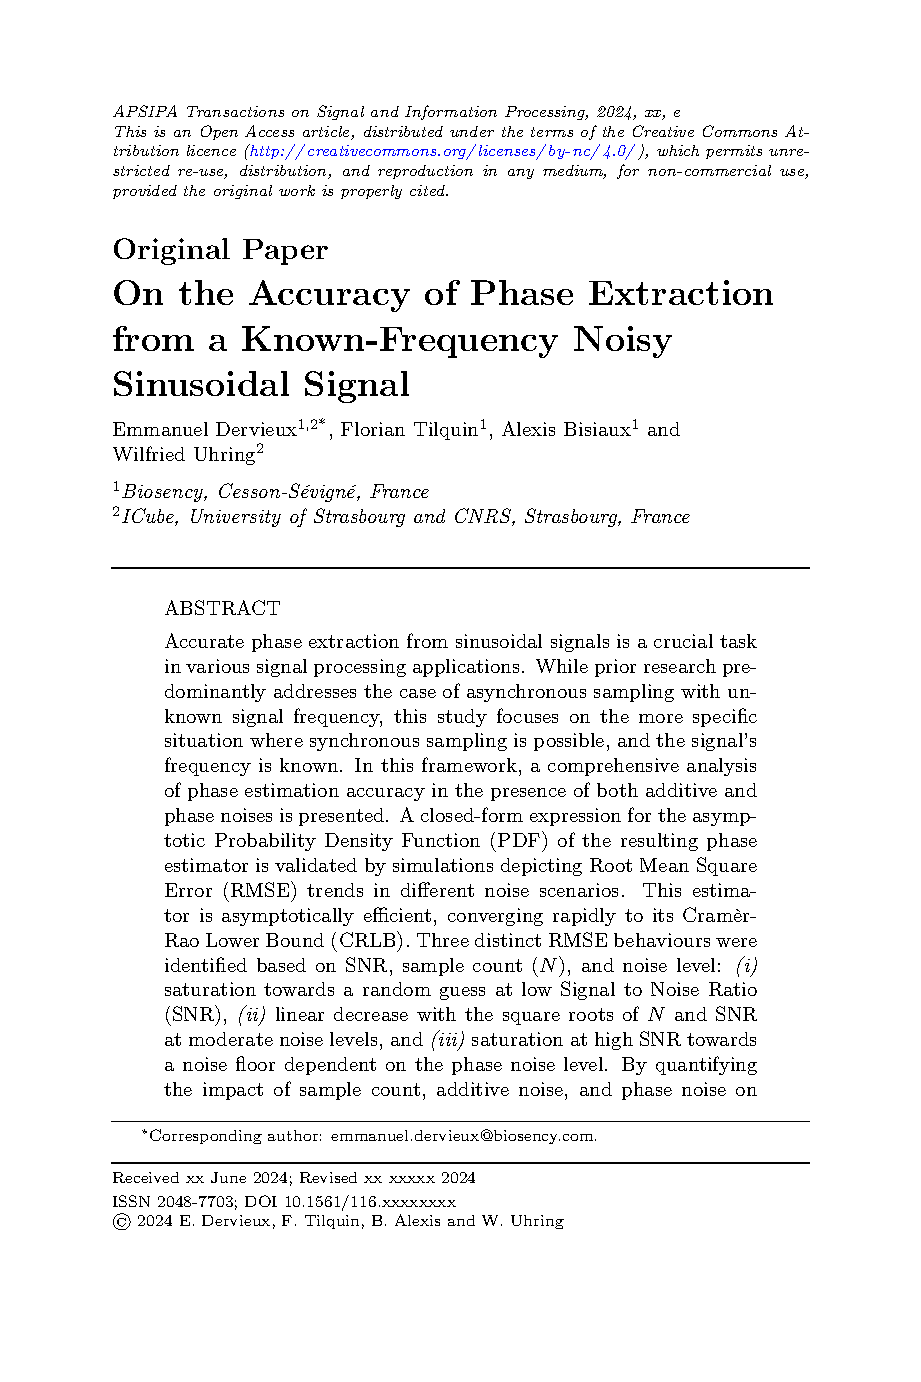
\includepdf[pages={1-}]{1_main_matter/dervieux_phase_apsipa.pdf}

\section{Conclusion}\label{sect:choos:conclusion}

The full range of \gls{co2} sensing techniques was first reviewed, extracting key figures of merit for each of the presented technique---Section~\ref{sect:choos:sensors_review}. Those techniques were then confronted to the exigencies of transcutaneous \gls{co2} sensing that were outlined in the previous chapter---Section~\ref{sect:choos:techno_choice}. In particular, \textit{(i)} the constraints for a small volume to surface ratio, \textit{(ii)} for a low drift, and \textit{(iii)} the presence of humidity at the skin oriented my choice towards dye-based \gls{co2} sensing. This sensing technique was then presented in great details in Section~\ref{sect:choos:dye_based}, which introduced both the sensing chemistry taking place inside the sensor and the optical sensing schemes that may be used to probe the latter. To this end, \gls{fdlr} was selected because of its inherent referencing---and thus independence towards fluctuation in \gls{led} intensity or photodiode sensitivity---and its reduced number of optical elements compared to ratiometric measurements, although at the cost of an increased complexity in signal processing. The subtleties of \gls{fdlr} were then discussed in Section~\ref{sect:choos:dye_based:dlr_theory}, concluding that an accurate phase measurement of the fluorescence signal was essential to its proper functioning.

This led me to conduct a thorough mathematical analysis of the influences of both additive and phase noise on the accuracy of the phase measurement of a sinusoidal signal---\ref{sect:choos:phase_mes}. This analysis resulted in a particularly interesting result in case the phase noise is not excessive, with the \gls{rmse} of the phase measurement following
\begin{equation}
	\text{\gls{rmse}}(\varphi_\text{mes}) = \frac{1}{\sqrt{N \cdot \text{\gls{snr}}}}
\end{equation}

The latter relation can then be used in real-world situations to adjust the illuminating power---influencing the \gls{snr}---or the duration of an acquisition---changing $N$---to dynamically make a compromise between power consumption and photobleaching on the one hand, and phase measurement accuracy on the other hand. With these theoretical foundations in place, we are now well prepared to tackle the next chapter, which covers the concrete implementation of the afore-mentioned principles into an \gls{fdlr} \gls{co2} sensor fit for transcutaneous sensing.